%\documentclass[journal=jpr,manuscript=article]{achemso}
\documentclass{article}
\usepackage[margin=0.5in]{geometry}
\usepackage{graphicx}
\usepackage{mathtools,amssymb}
\usepackage{color}
\usepackage[english]{babel}
\usepackage{authblk}
\usepackage{url}
%\usepackage{soul}
\usepackage[ruled,vlined,linesnumbered]{algorithm2e}
\usepackage{algorithmic}


%\graphicspath{{figs/}}  Store figures at the level of the main doc
\newcommand{\argmax}{\text{argmax}}
\newcommand{\todo}[2]{{\color{red} {\bf TODO-#1}: #2}}
\newcommand{\comment}[2]{{\color{blue} {\bf Comment-#1}: #2}}
\newcommand{\correction}[2]{{\color{red} \st{#1} }{\color{red} #2}}
%\newcommand{\correction}[2]{#2}  % Use this to make a document with hiding track changes.

%\usepackage[backend=biber,style=nature,articletitle=false]{biblatex}
%\usepackage[backend=biber,style=nature]{biblatex}
%\addbibresource{bibliography.bib}

%\usepackage[backend=biber]{biblatex}
%\usepackage{natbib}
%\addbibresource{bibliography.bib}
\newcommand{\pe}[0]{\mathrel{{+}{=}}}

\usepackage{setspace}
\doublespacing
%\newcommand*{\DOUBLEBLINDREVIEW}{} %Uncomment to hide author information for double-blind peer review


\author{Andrey Borevsky}
\author{Attila Kertesz-Farkas$\ast$}
\affil{Laboratory on AI for Computational Biology, Faculty of Computer Science, HSE University,  11 Pokrovsky Bvld., Moscow 109028, Russian Federation}
%\email{akerteszfarkas@hse.ru}
%\phone{+7 (499) 152-07-41}

\title{Utilizing exact p-values for improved classification and accurate false discovery rate control}

\begin{document}

\maketitle

\begin{abstract}
Exact p-value (XPV)-based methods for dot product-like score functions ...


\end{abstract}
\textbf{Key words:} Exact p-values, empirical p-values, False discover rate control, classification, score calibration
\section{Introduction}
The performance of machine learning methods, classifiers are typically evaluated with accuracy, ROC, and precision/recall metrics. However, in certain applications, such as those in biomedical area, False discovery rate (FDR) control is preferred. Several methods have been proposed to control FDR at a certain, user-controlled level. Perhaps, the most well-known FDR control method is the Benjamini-Hochberg protocol (BHP). Some FDR control methods rely on knock-off \todo{akf}{Check these knock off methods} or decoy samples. Perhaps, other types of FDR control methods rely on accurate p-values associated to each prediction.

The false discovery rate is the expected proportion of falsely classified data, whereas a false discovery is a data instance that is misclassified. 

The aim of this study:
\begin{itemize}
	\item Demonstrate the accuracy of the empirical p-values,
	\item Accurate FDR error control can be achieved without class labels on the test data.
	\item it can be used to detect distribution shift in the test data. 
\end{itemize}

\section{Methods}


It is important to keep it in mind that methods reporting p-values using either analytical models (such as normal distribution) or some empirical methods are just merely estimations/approximatinos of the true but unknow p-values. If a p-value estimation method systematically produces more significant p-values, i.e. smaller numbers, than the true (but unknown) p-values, then it is called a liberal or optimistic; if it systematically produces less significant p-values, i.e. larger numbers than the true p-values, it is called a conservative estimation. Luckily, there is a way to asses the bias in p-values. It is known that, sampling from a distribution, the corresponding p-values are uniformly distributed. In order to show this, let us assume we are given a continuous, cumulative distribution function $F_X(X)$ and it is invertible, i.e. $F_X^{-1}$ exists. We want to show that, the p-values $Z = 1-F_X(X)$ are uniformly distributed, that is $F_Z(X)$ is uniformly distributed. Note that $Z\in [0,1]$. For the uniform distribution on $U\sim U_{[0,1]}$, we also have $1-U\sim U_{[0,1]}$ uniformly distributed, furthermore $P(U\le u)=u$ and $P(U>u) = 1-u$ for any $u\in[0,1]$. Thus,
\begin{equation}
	F_Z(u)=P(Z \le u) = P(1-F_X(X)\le u)= 1-P(X\le F_X^{-1}(u))=1-F_X(F_X^{-1}(u))=1-u.
\end{equation}

Therefore, one can draw a QQ plot of the p-values against the theoretical uniform distribution for visual verification.

In this paper, we propose to use the training data to produce a null distribution $N_0$ and for a given prediction score $s$ we define the p-value as $P_{N_0}(s)=\frac{|\{x\mid x>s, x \in N_0\}|}{|N_0|}$, where $|.|$ denotes the cardinality of set. Using these p-values, the false discovery rates can be controlled, for instance, with using the Benjamini-Hochberg protocol. We note that, the aim of this study is the investigation of the p-values, and we will use the BHP as a tool to demonstrate that these empirical p-values can be used to control the FDR; however, other FDR control methods could be used, for instance, for correlated p-values, etc. 

\todo{AKF}{the introduction and the methods sections are quite rudimentary. The need rearrangement.}

The FDR control could potentially be carried out by controlling the FDR on the training data at a user defined $\alpha$ level and selecting the corresponding score as a threshold $t$. A test data achieving a prediction score less than threshold $t$ could be rejected, etc. The major issue with this approach is that, it does not adapt neither to the class distribution nor to the data distribution shifts. the method we propose here adapts to when the proportion of the positive and negative classes changes, or it can visually detect data distribution shifts. 


\section{Data and methods}
\subsection{MNIST dataset}
The ubiquitously known MNIST dataset is a rich collection of handwritten digits, becoming a baseline for any classification task nowadays. It contains 60k samples for the training stage and only 10k for the test, where all classes (from 0 to 9) are evenly distributed. Also to be mentioned is the strict normalization of the digits in the image in terms of size and centering, so the algorithms receive unified examples as input.
\subsection{Logistic regression classifier}
We have accomplished a major part of the research's first stages through the standard logistic regression model. It comprised a single linear layer renewed by Adam optimizer with a learning rate equal to 0.01 and a BCEWithLogitsLoss cost function. The motivation was straightforward: if we find ourselves able to ameliorate a particular quality of an elementary model on the resolvable MNIST dataset, then we could extend our approach to more comprehensive tasks and algorithms.

\subsection{Convolutional neural network classifier}
Nevertheless, all the presented figures correspond to the usage of a more powerful CNN model. It consists of two convolutional 2d layers, each followed by a rectifier activation function. The output layer is presented by a simple linear unit, providing as much classes, as it was initialized by the user.   


\section{Results}

\begin{figure}
	\centering
	\begin{tabular}{ccc}
 		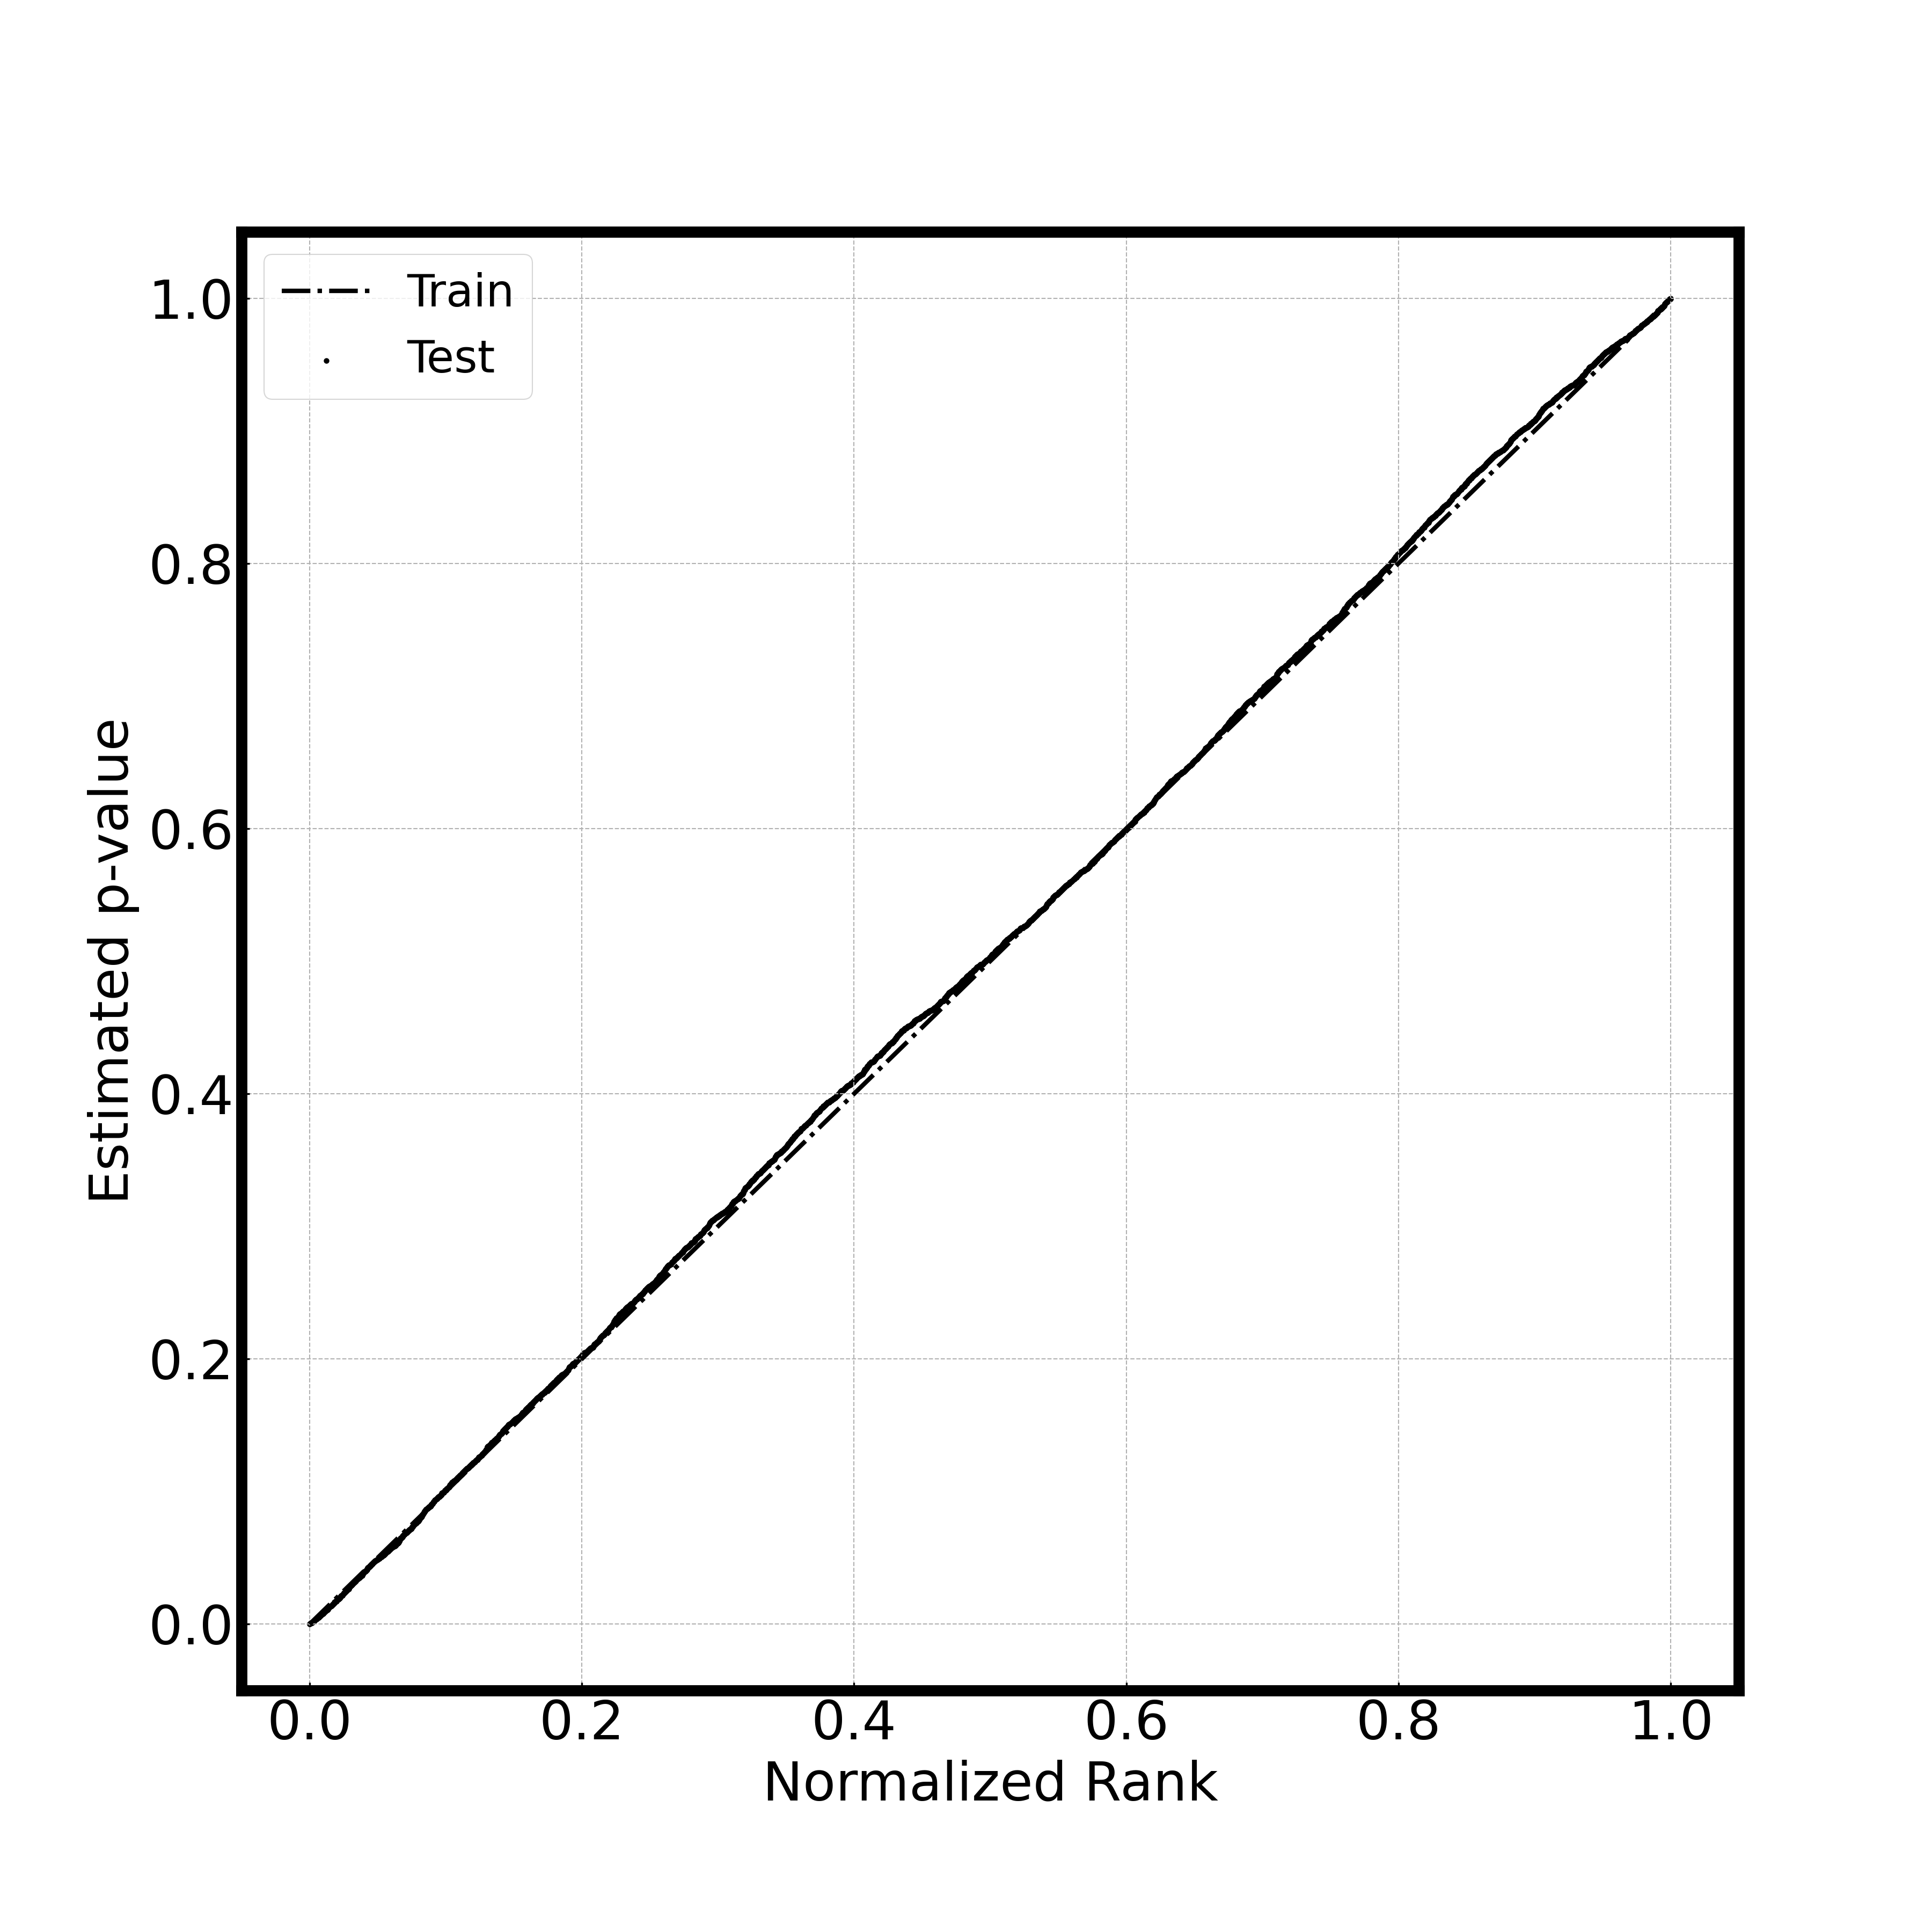
\includegraphics[width=2in]{img/cnn_QQ_with_labels.png} &
		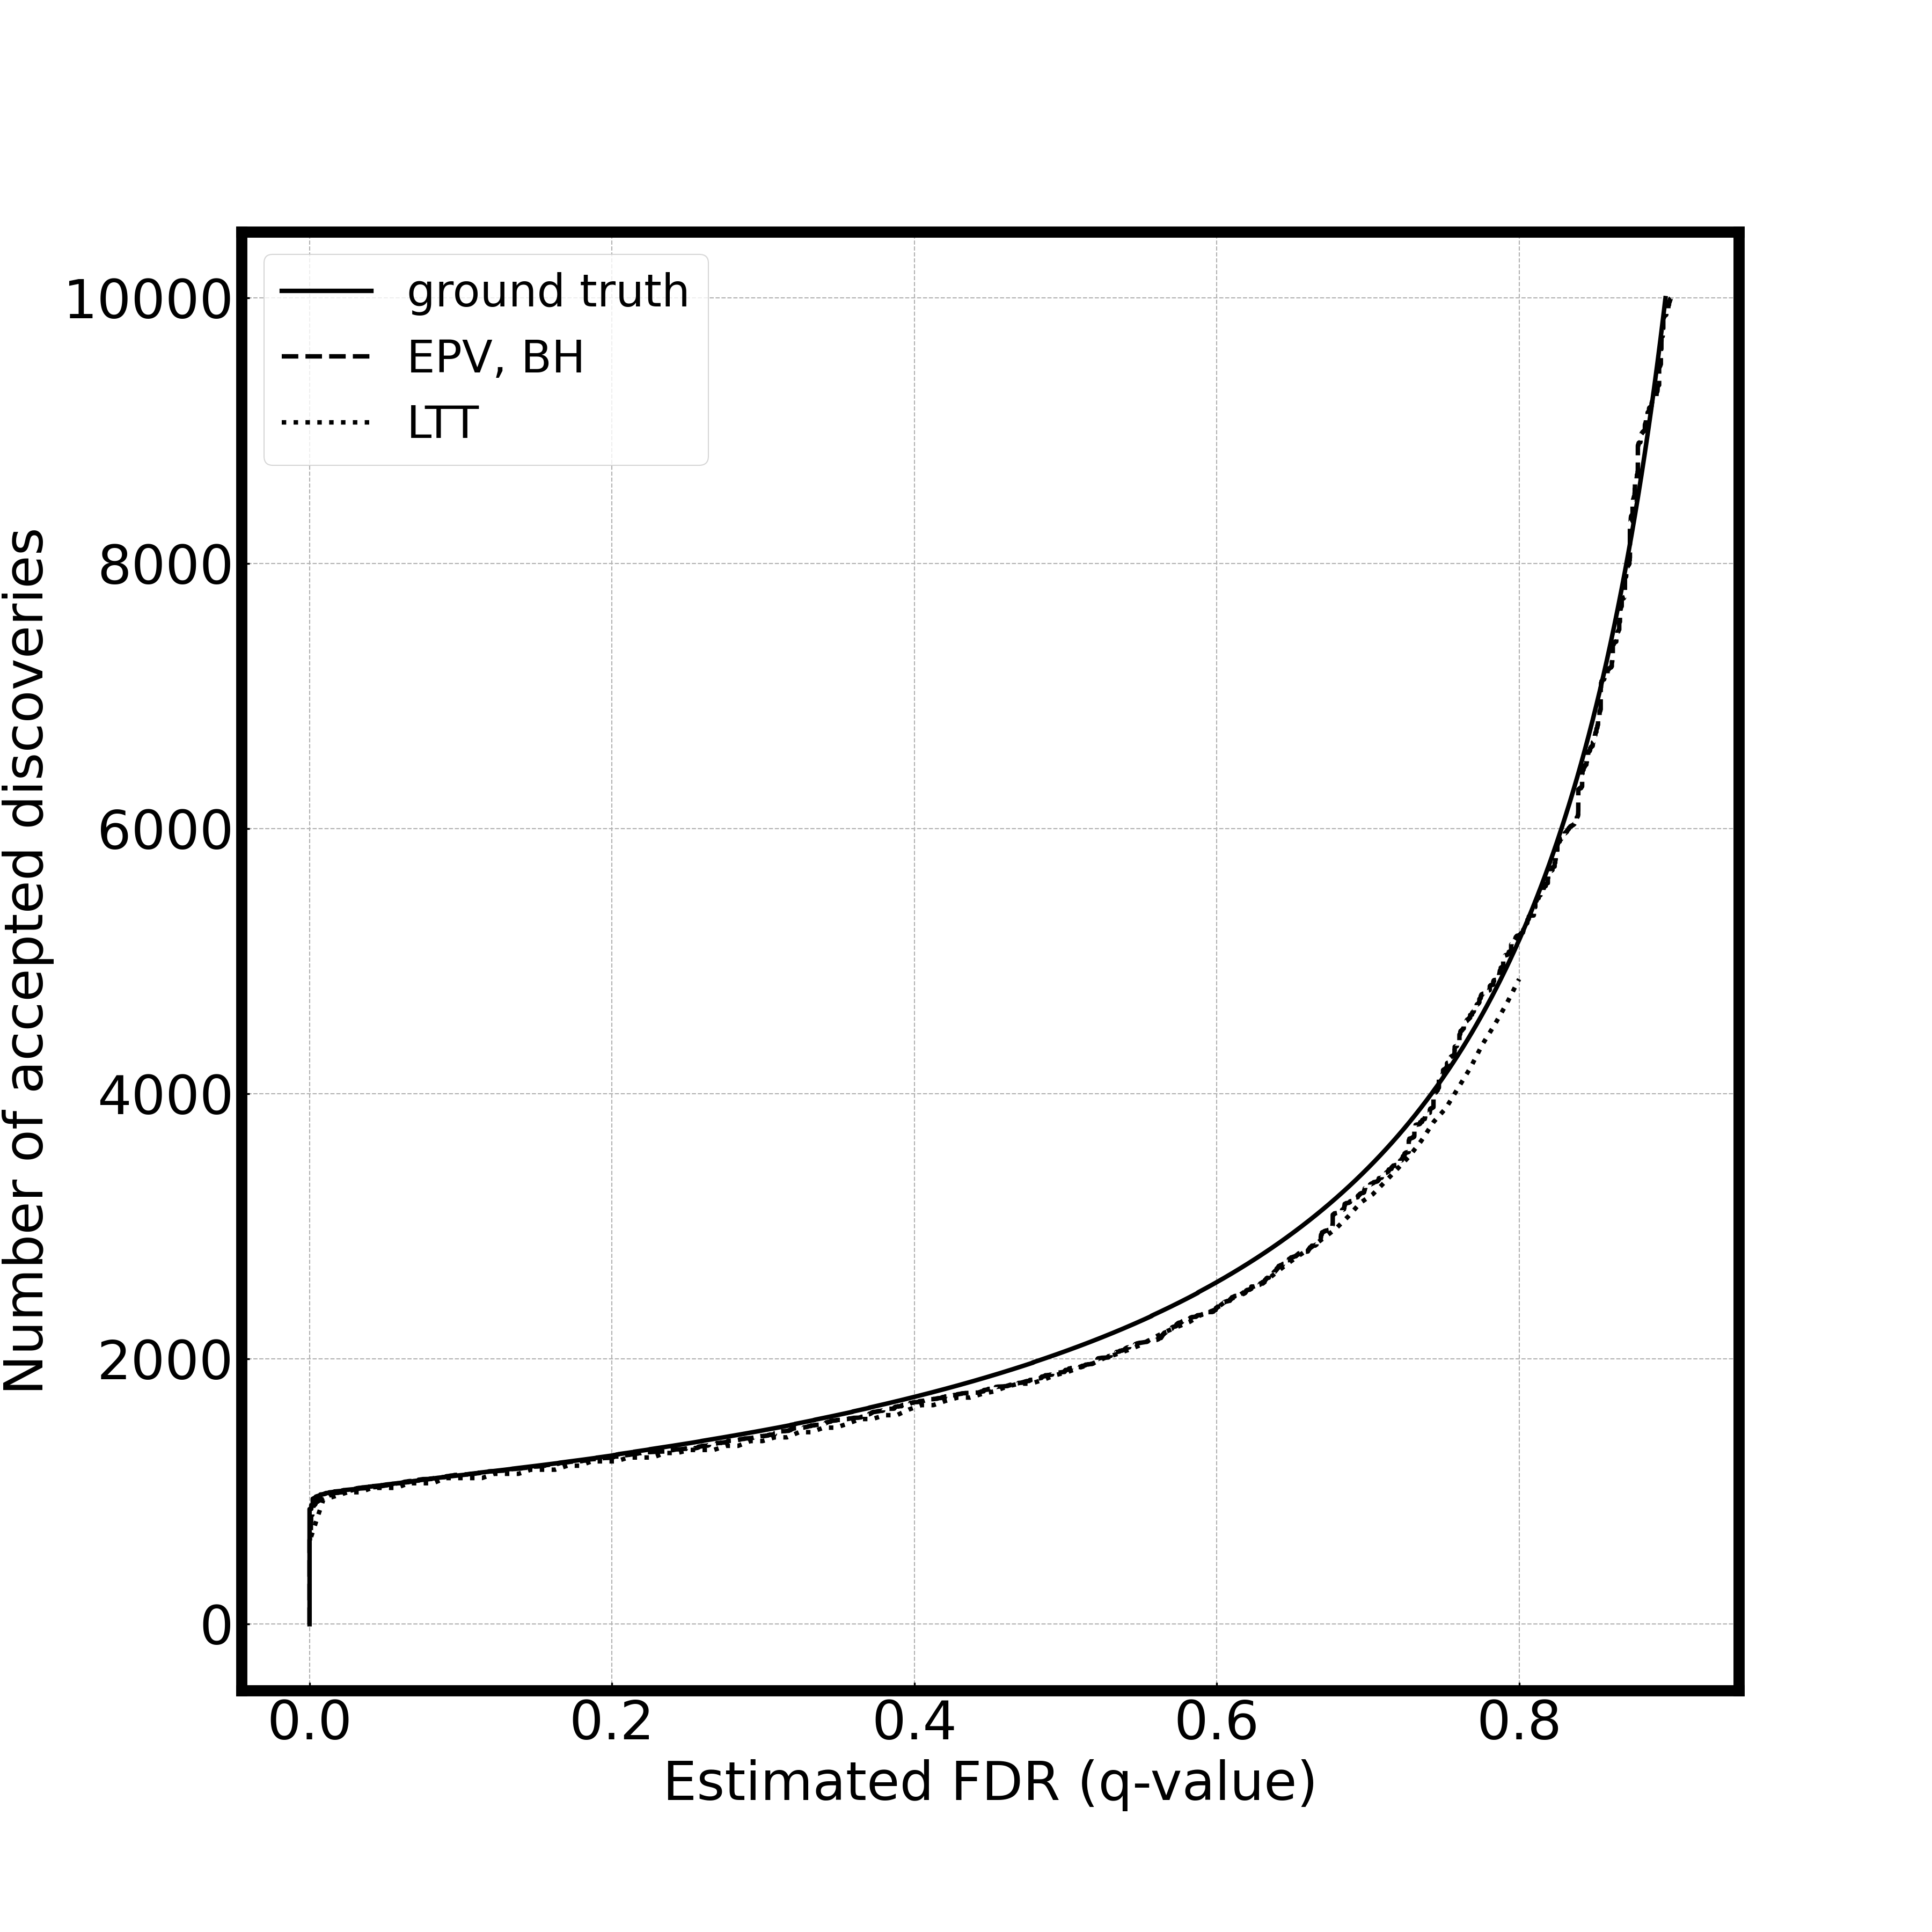
\includegraphics[width=2in]{img/cnn_test_pred_with_labels.png} & 
            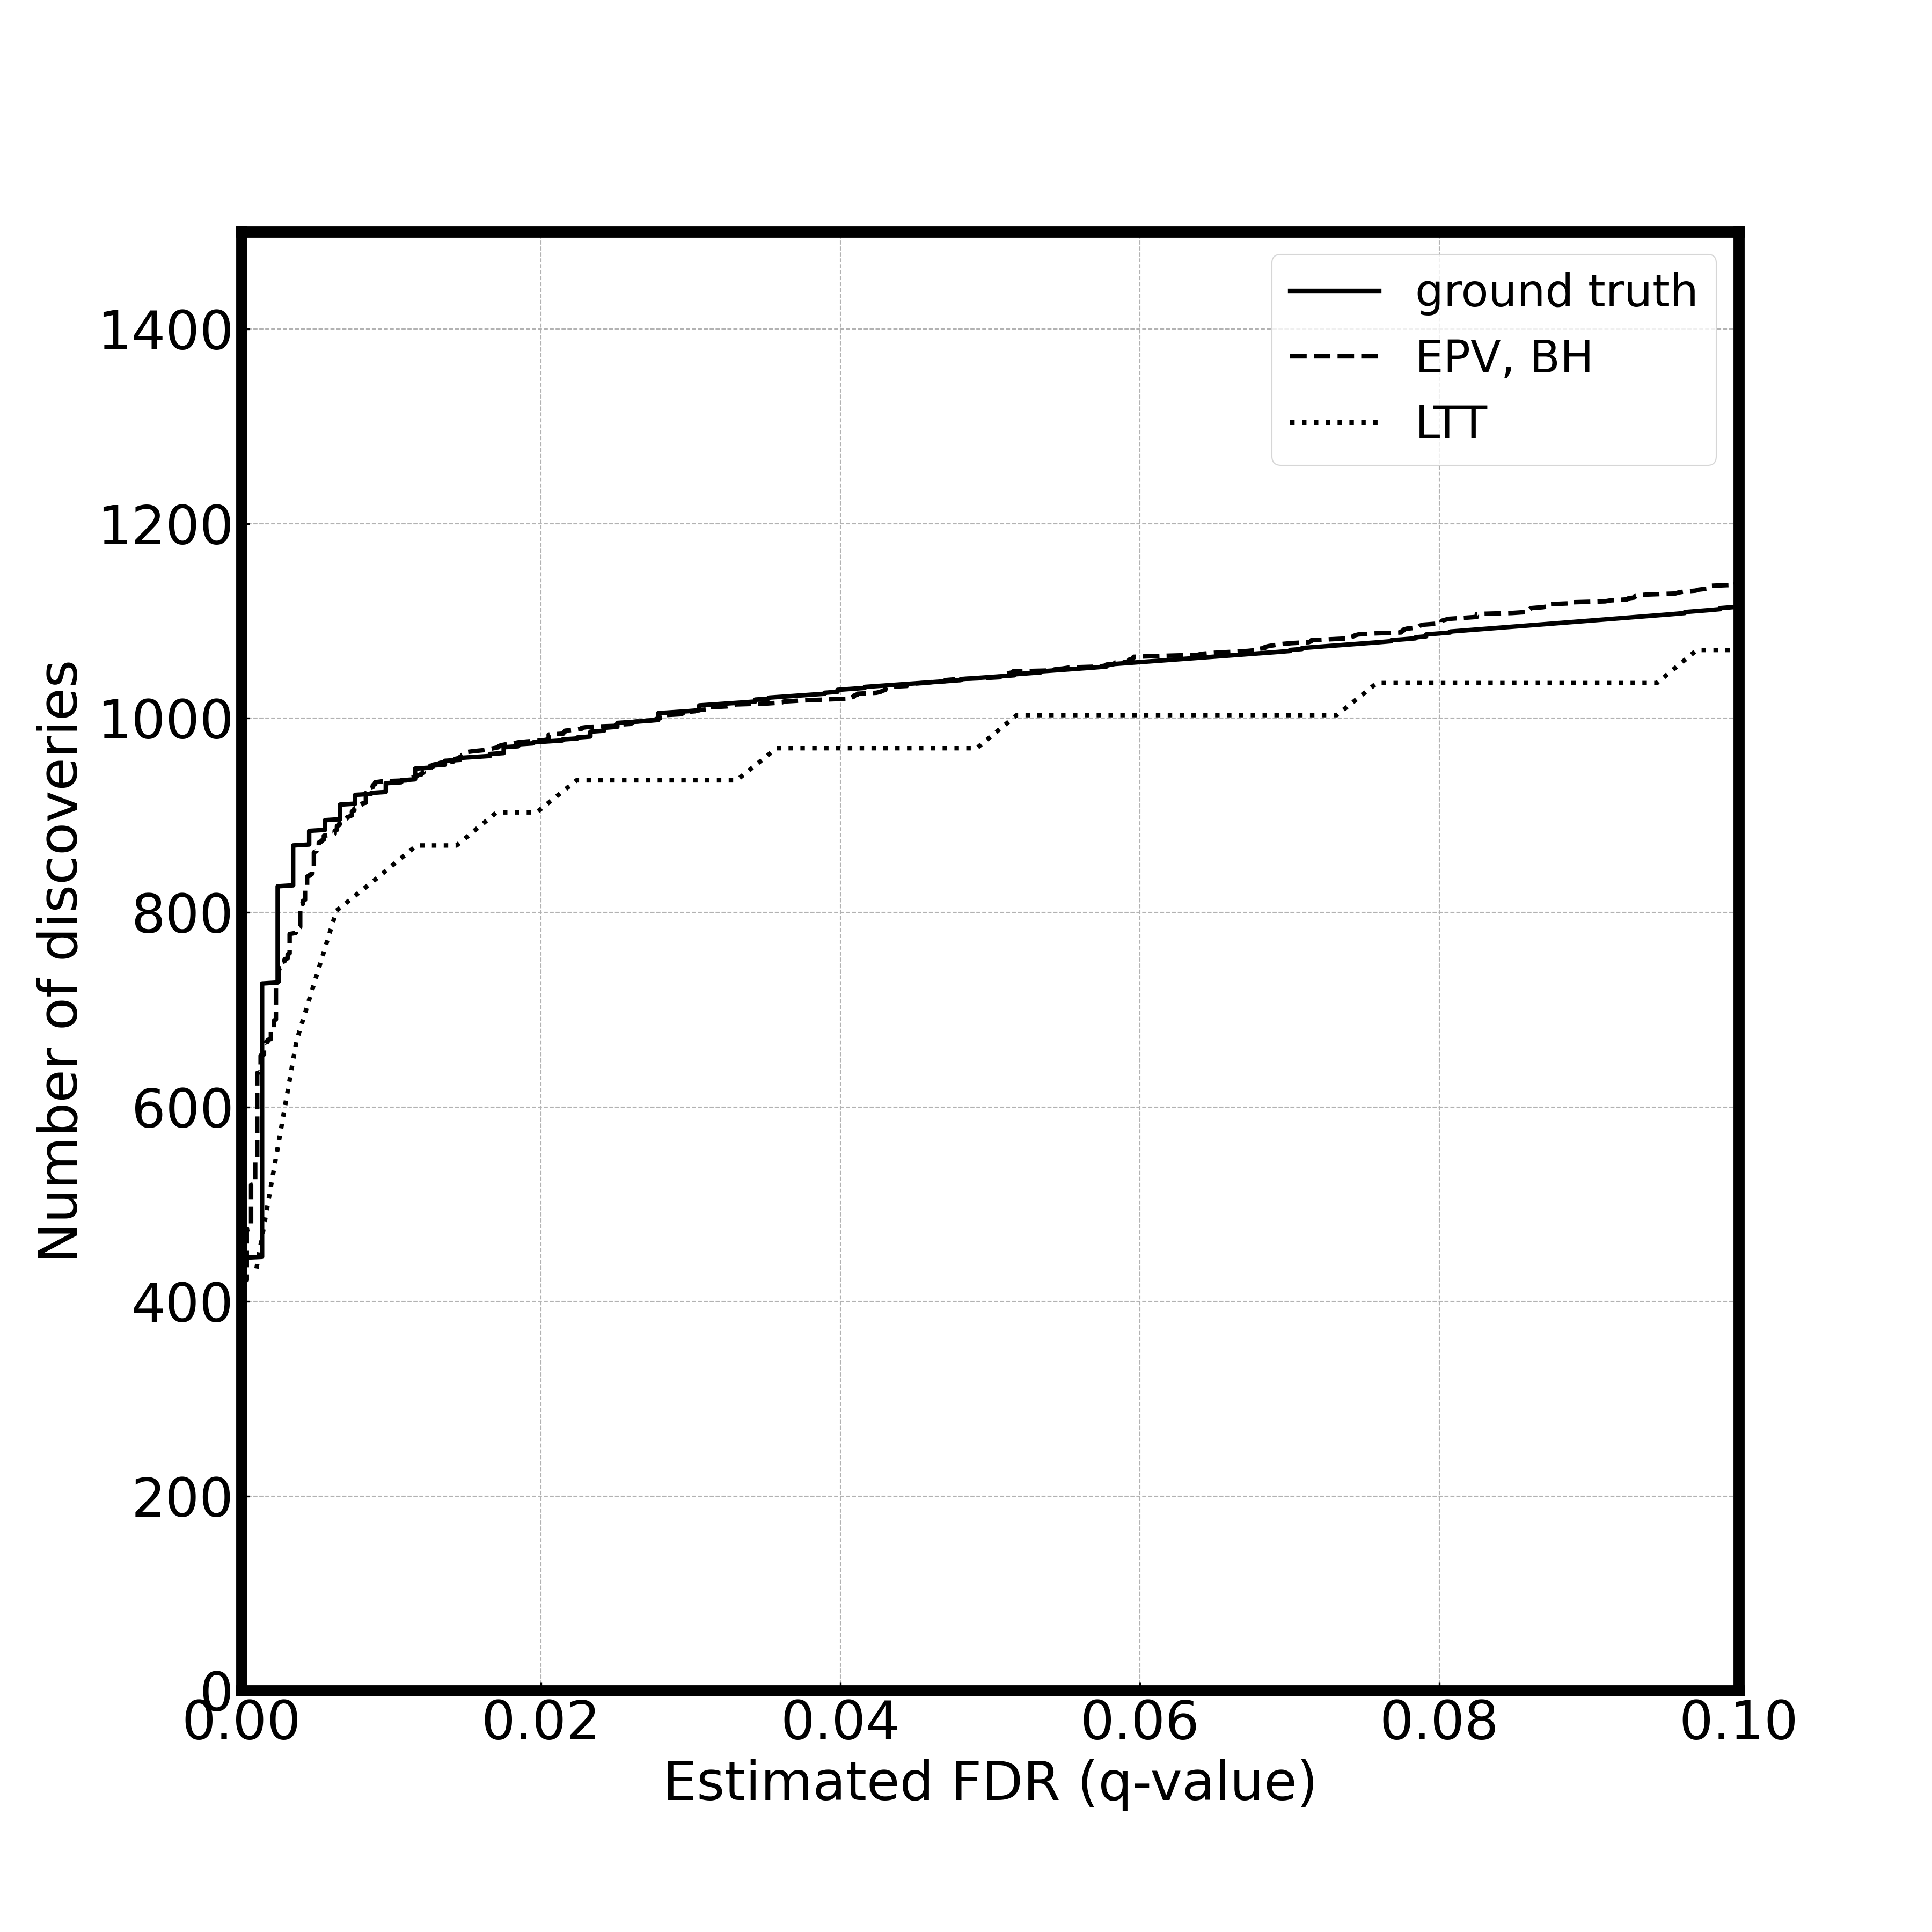
\includegraphics[width=2in]
            {img/cnn_test_pred_with_labels_loc.png}
		\\
		%    \includegraphics[width=3in]{digestion.pdf} & \includegraphics[width=3in]{cleavages.pdf} \\		
		A & B & C\\
            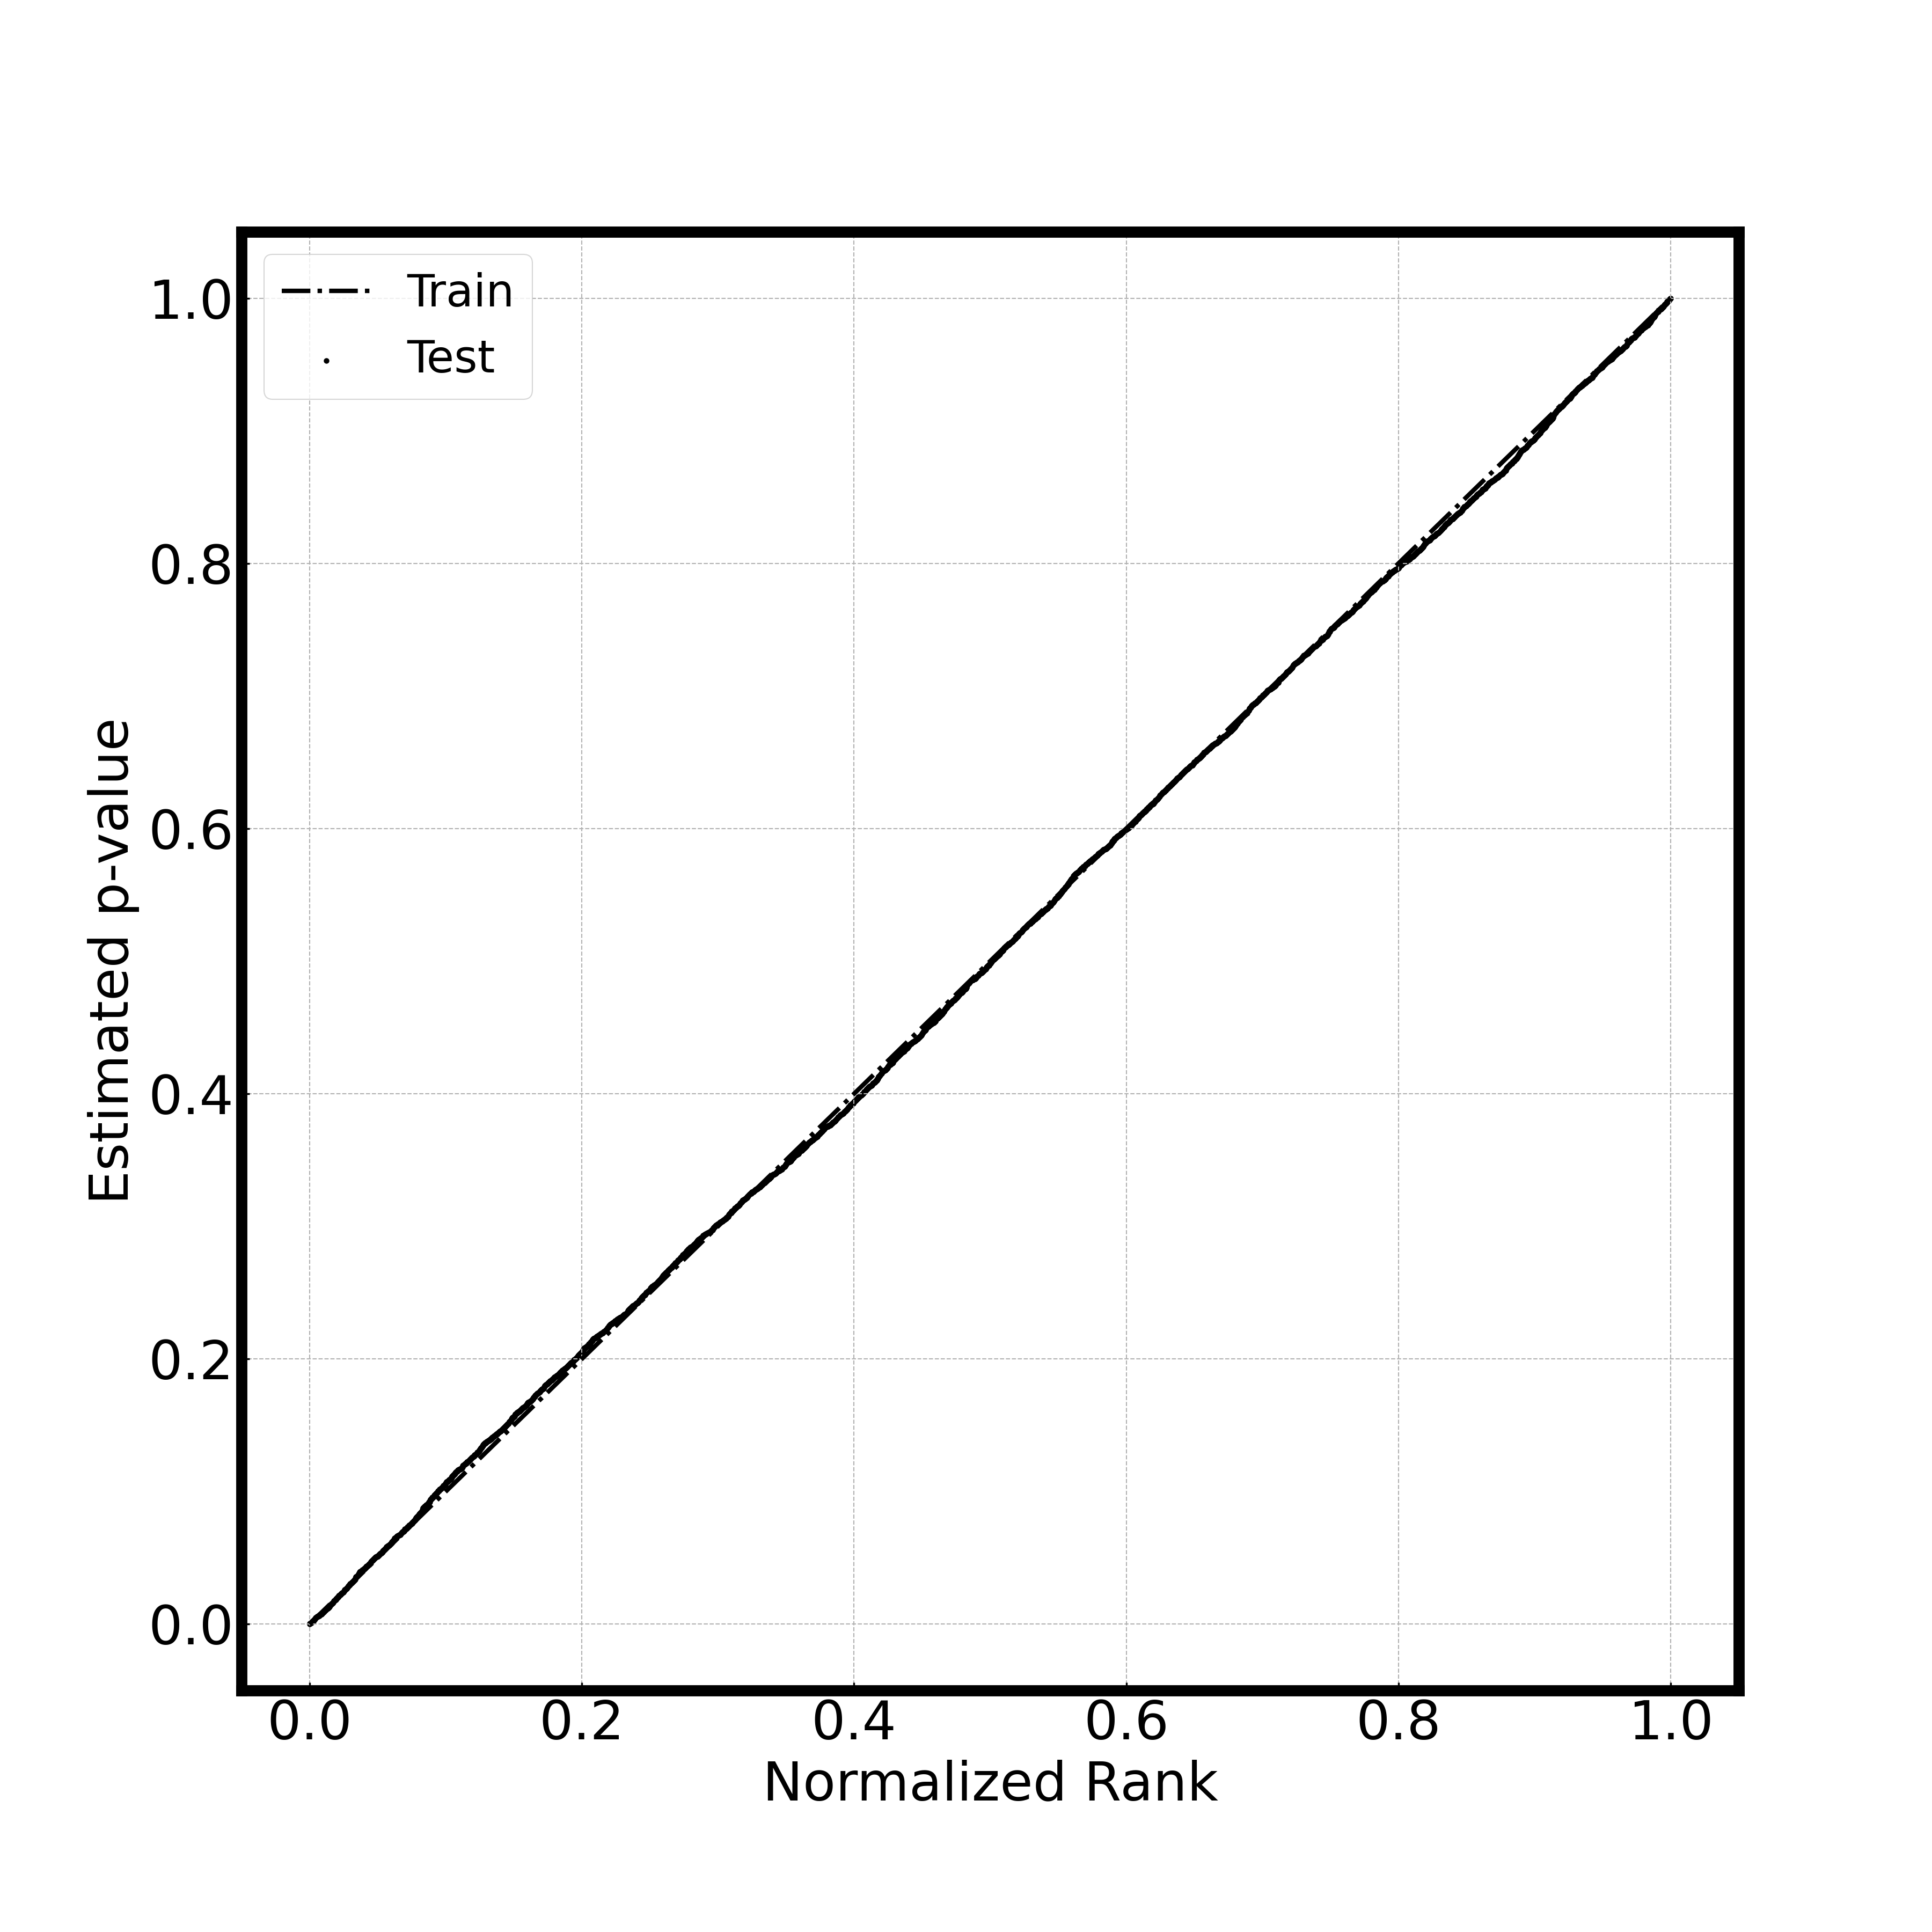
\includegraphics[width=2in]{img/cnn_QQ_no_labels.png} &
		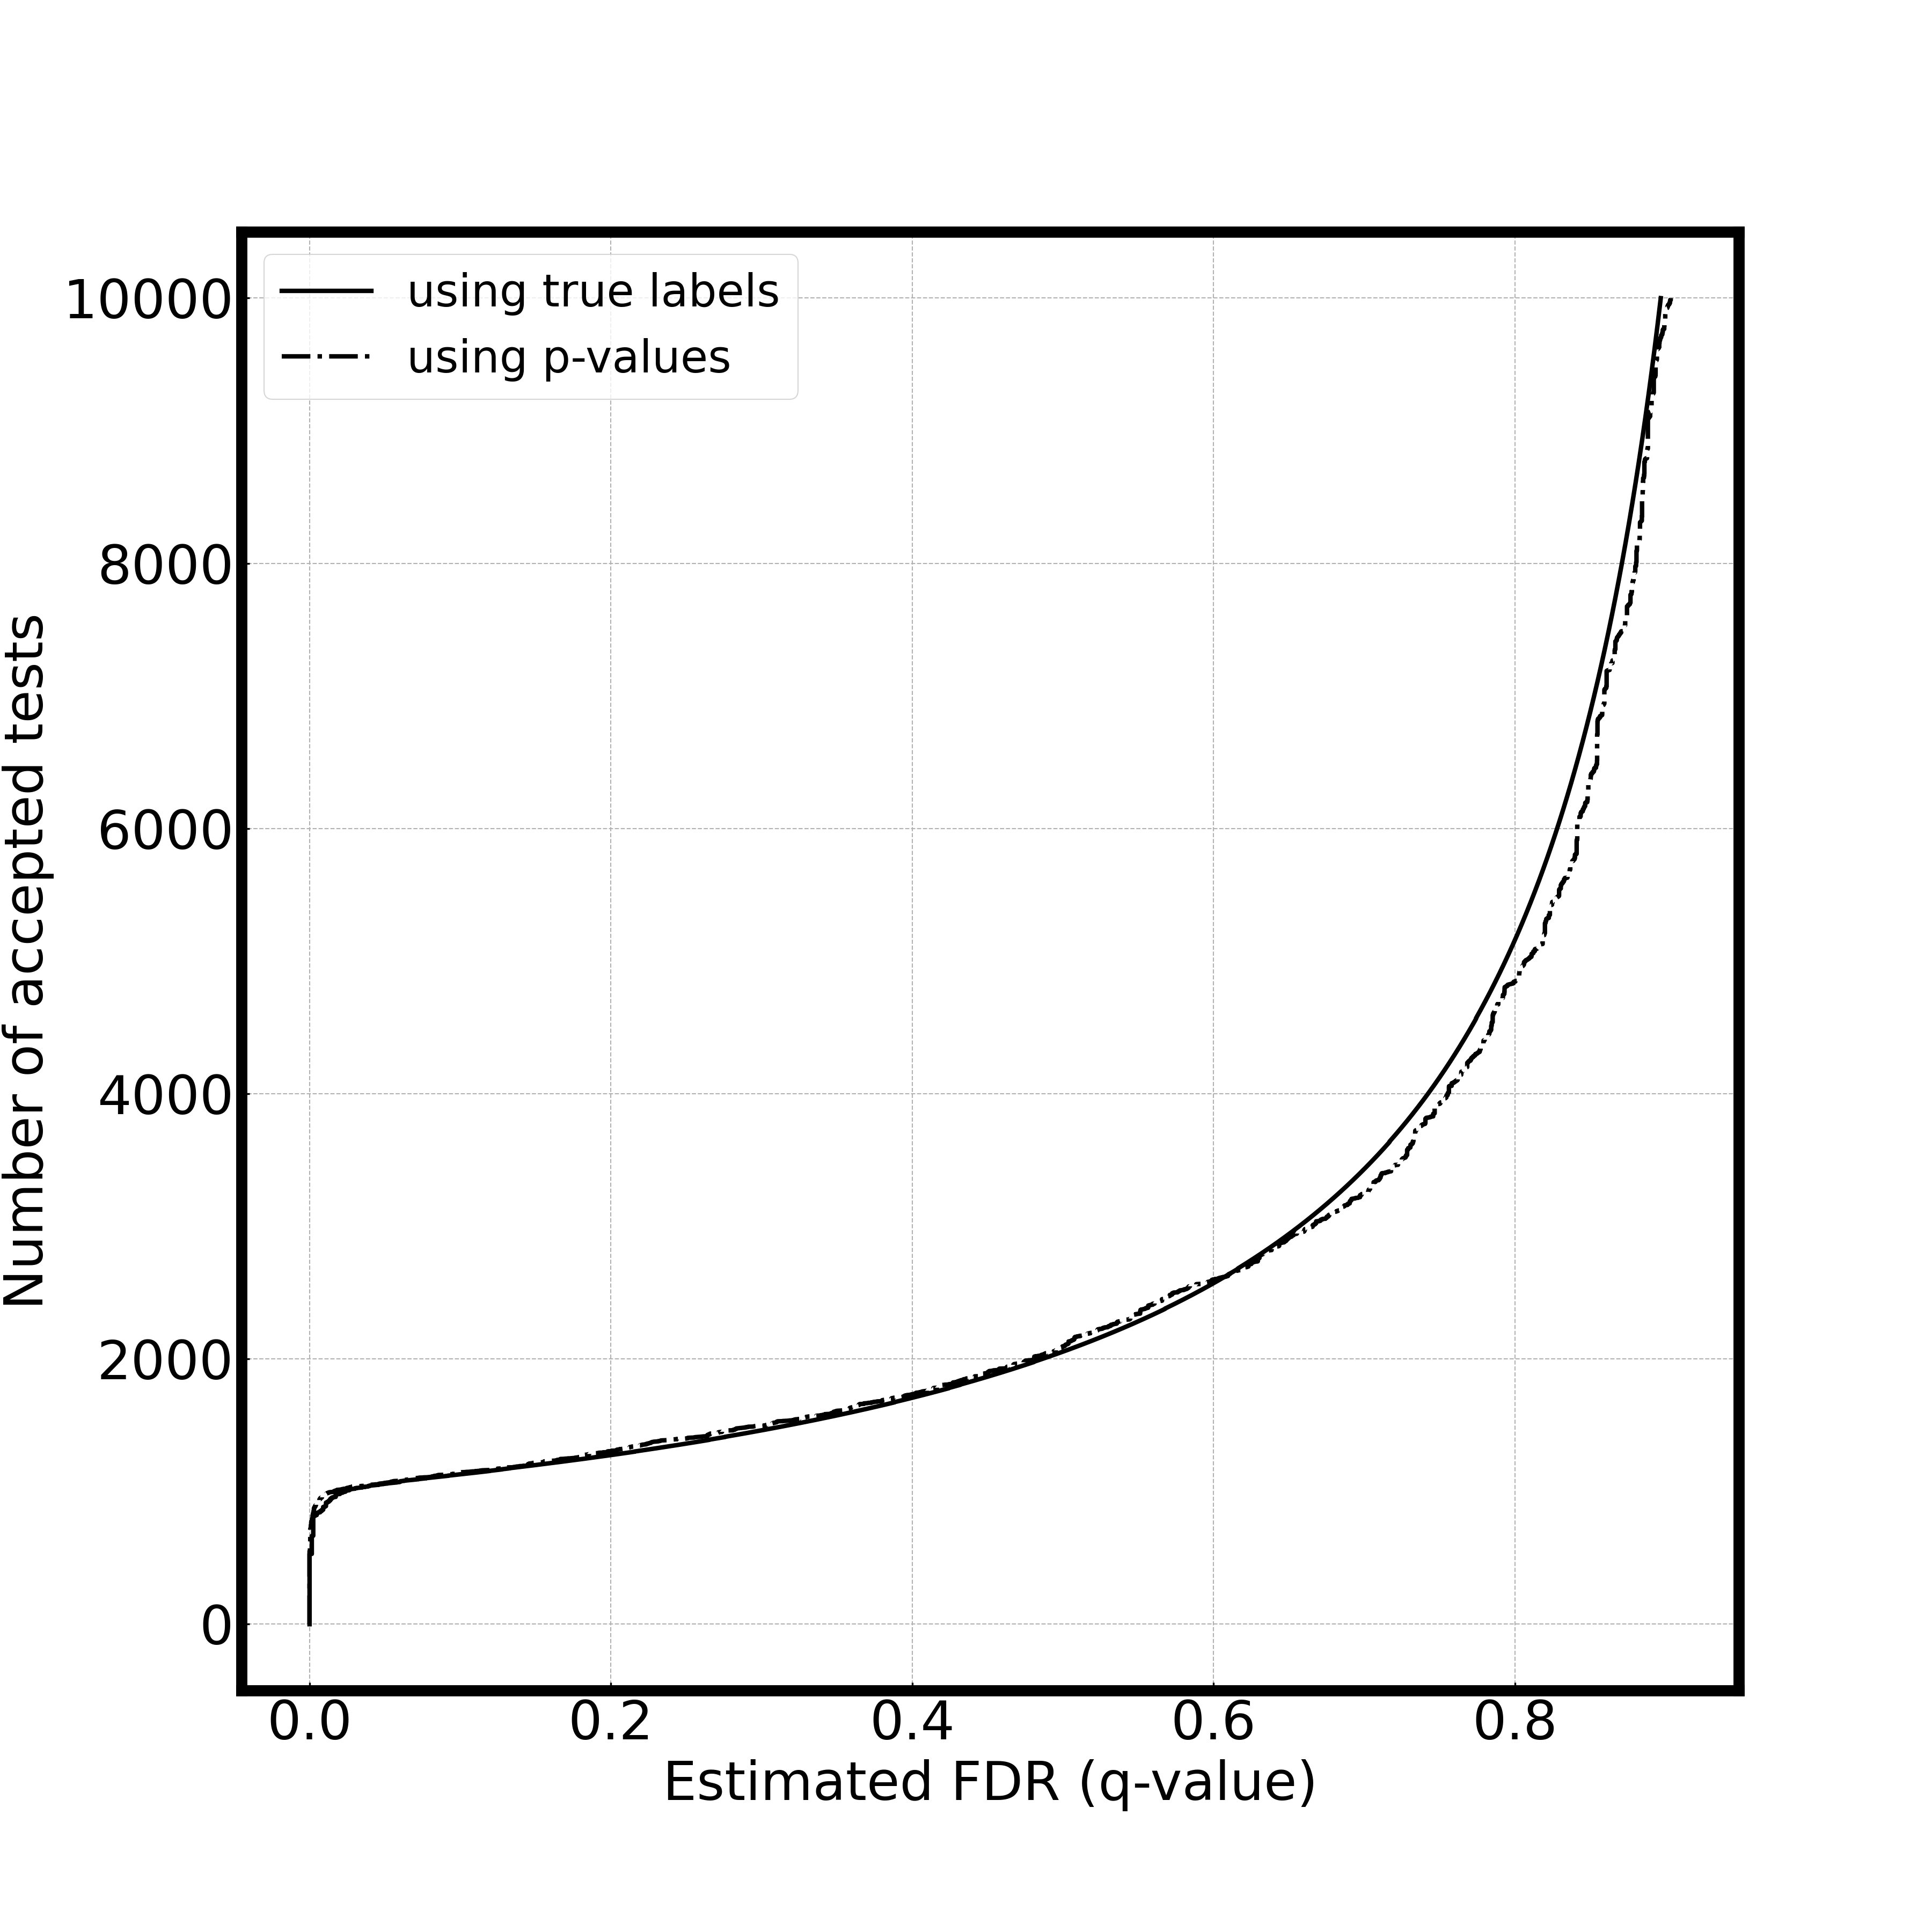
\includegraphics[width=2in]{img/cnn_test_pred_no_labels.png} &  
            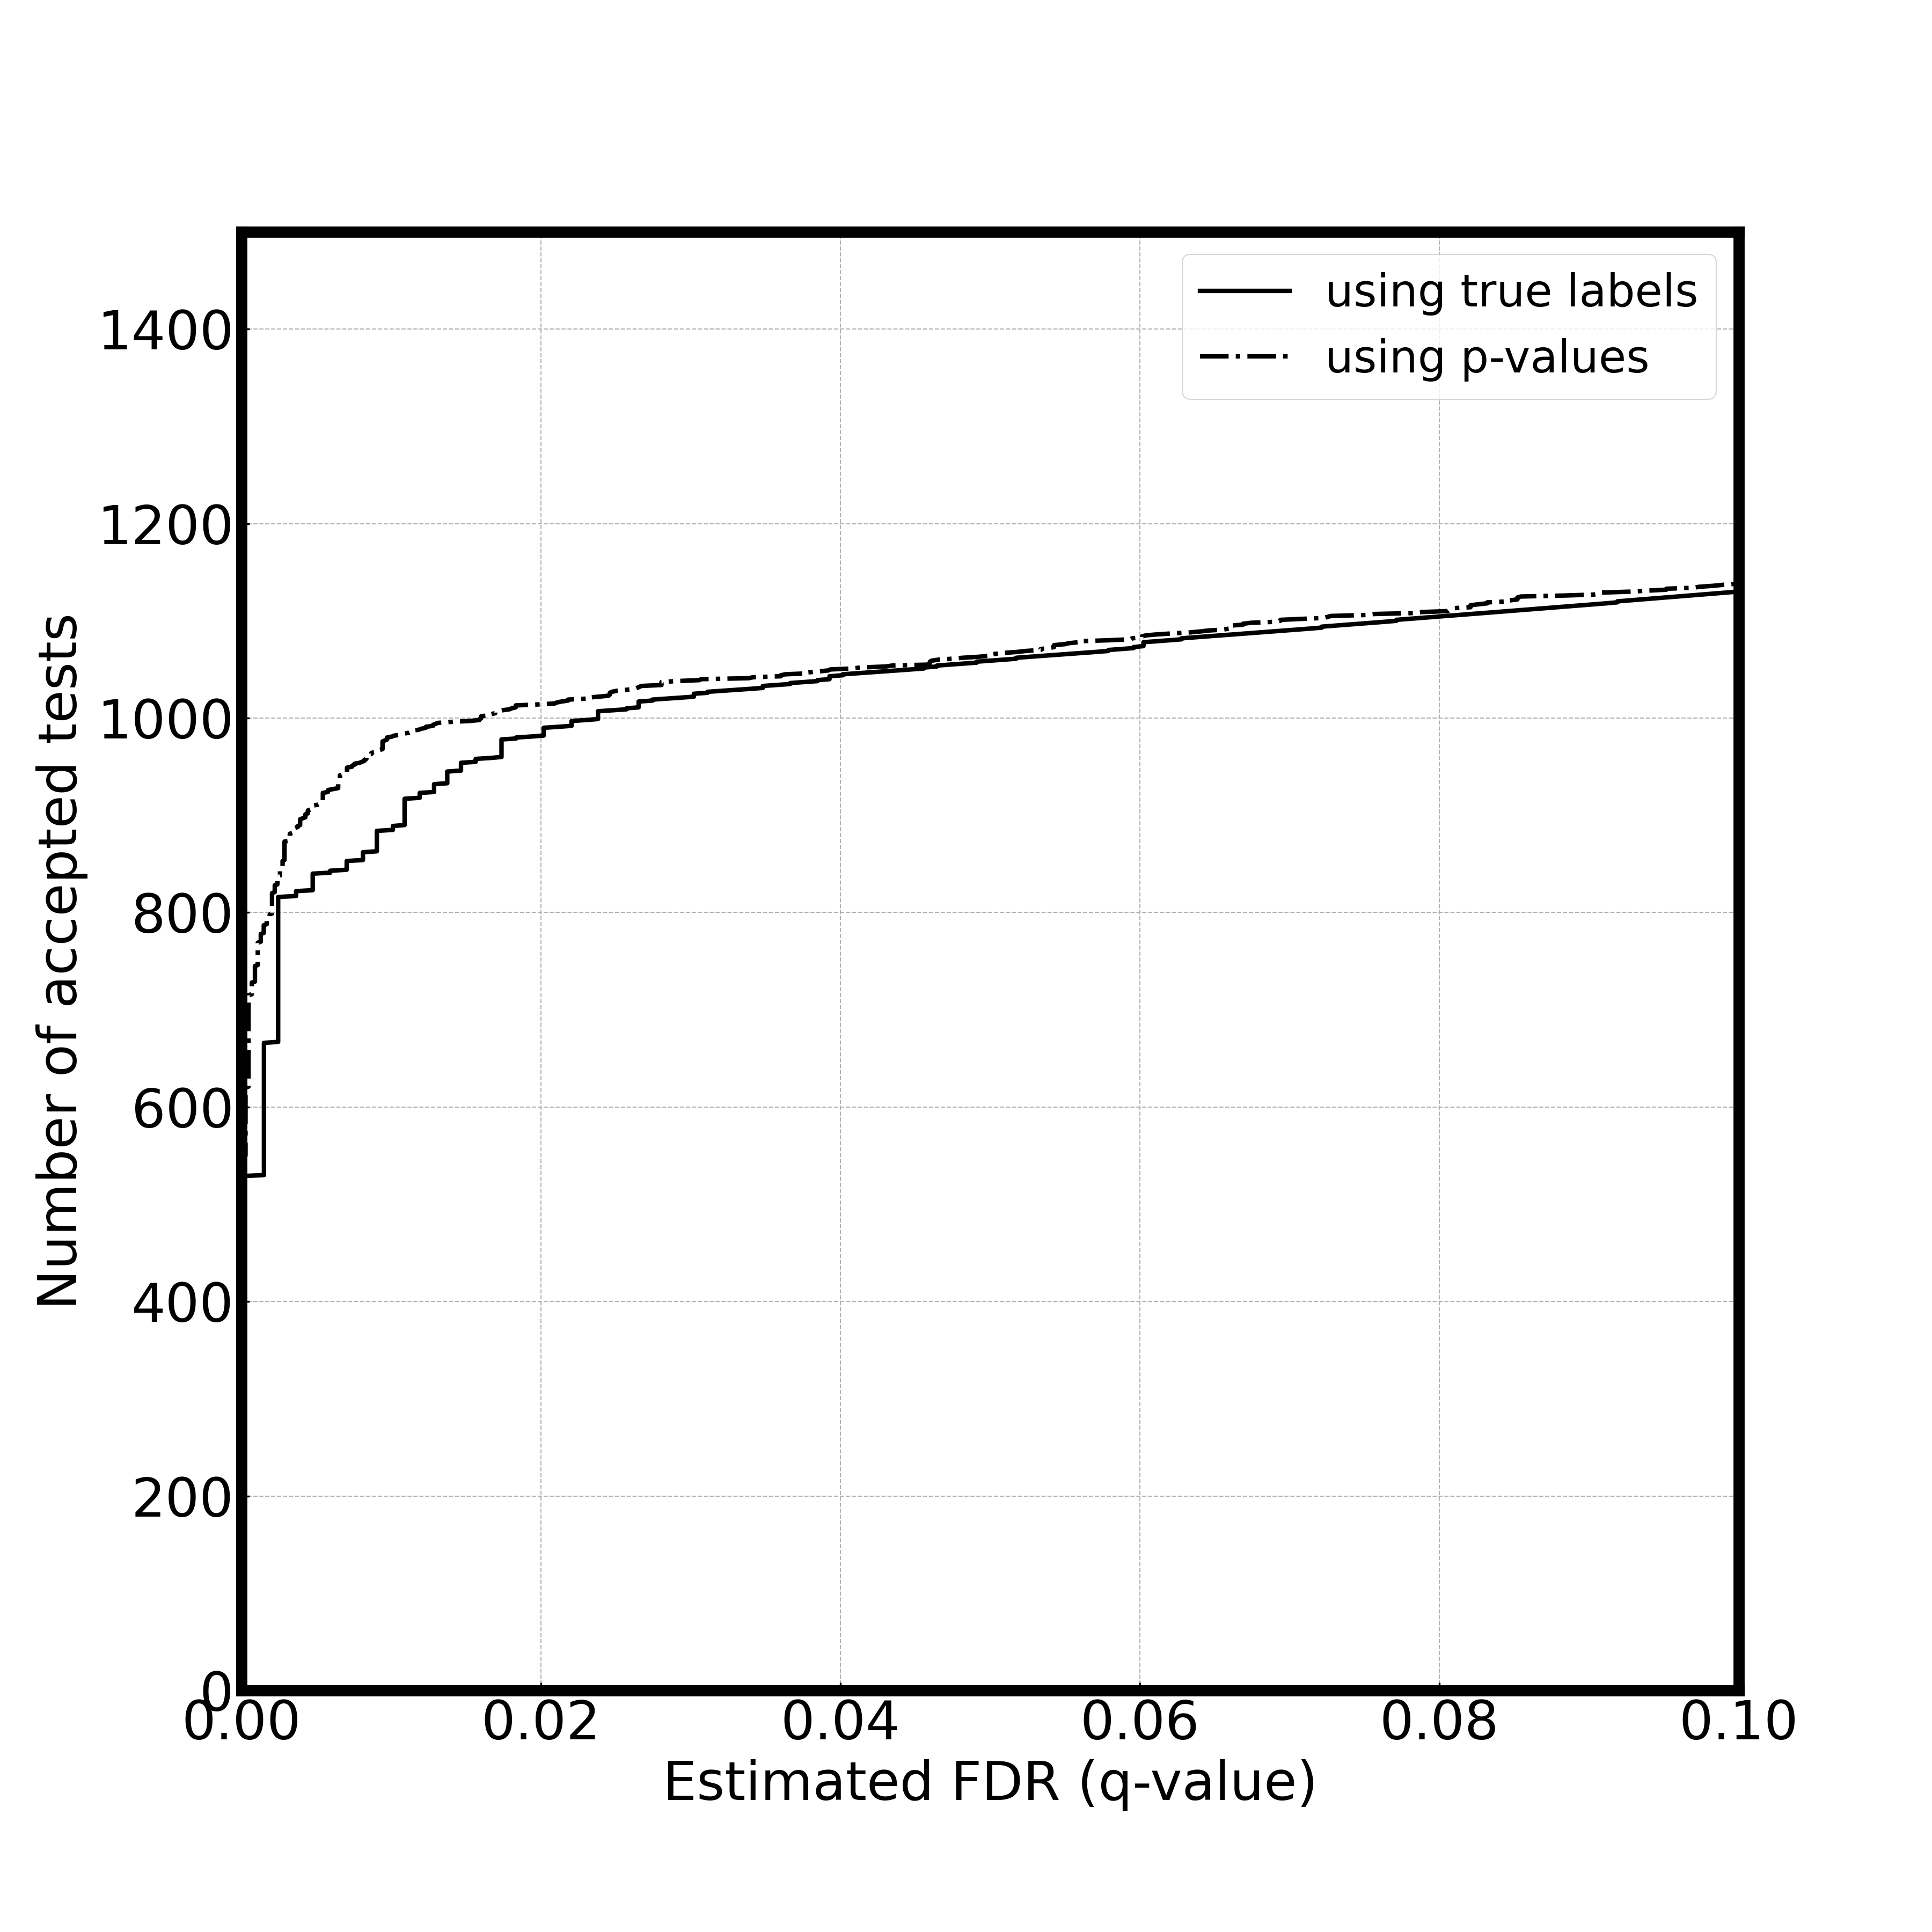
\includegraphics[width=2in]{img/cnn_test_pred_no_labels_loc.png}  \\
		D & E & F \\
	\end{tabular}
	\caption{{\bf FDR control with p-values.}
		(A) a QQ plot of the p-values obtained with using negative training data. (B) The number of trusted classifications as a function of the FDR when it is controlled with true labels (red line) and with controlled with BHP (black line) using the p-values from panel (A). $\pi_0$ is estimated on the test data.
		(A) a QQ plot of the p-values obtained with using training data classified as negative. (B) The same as panel (B), but using p-values from panel (C).
	}
	\label{fig:examples}
\end{figure}  

\subsection{p-values for binary classification}

For binary classification, one can use the prediction scores negative training data as a null distribution. The BHP requires the ratio of the positive (null hypothesis) and the negative (alternative hypothesis) classifications denoted as $\pi_0$. In our case, $\pi_0$ is estimated by the proportion of the negative classification among all classifications in the test data.  

We arbitrarily chose the class "2" as a positive class from the MNIST data, and all other data corresponding to other classes were treated as negative data. \todo{AB}{Use can chose other target class}.
  


\begin{figure}
    \centering
	\begin{tabular}{cc}
		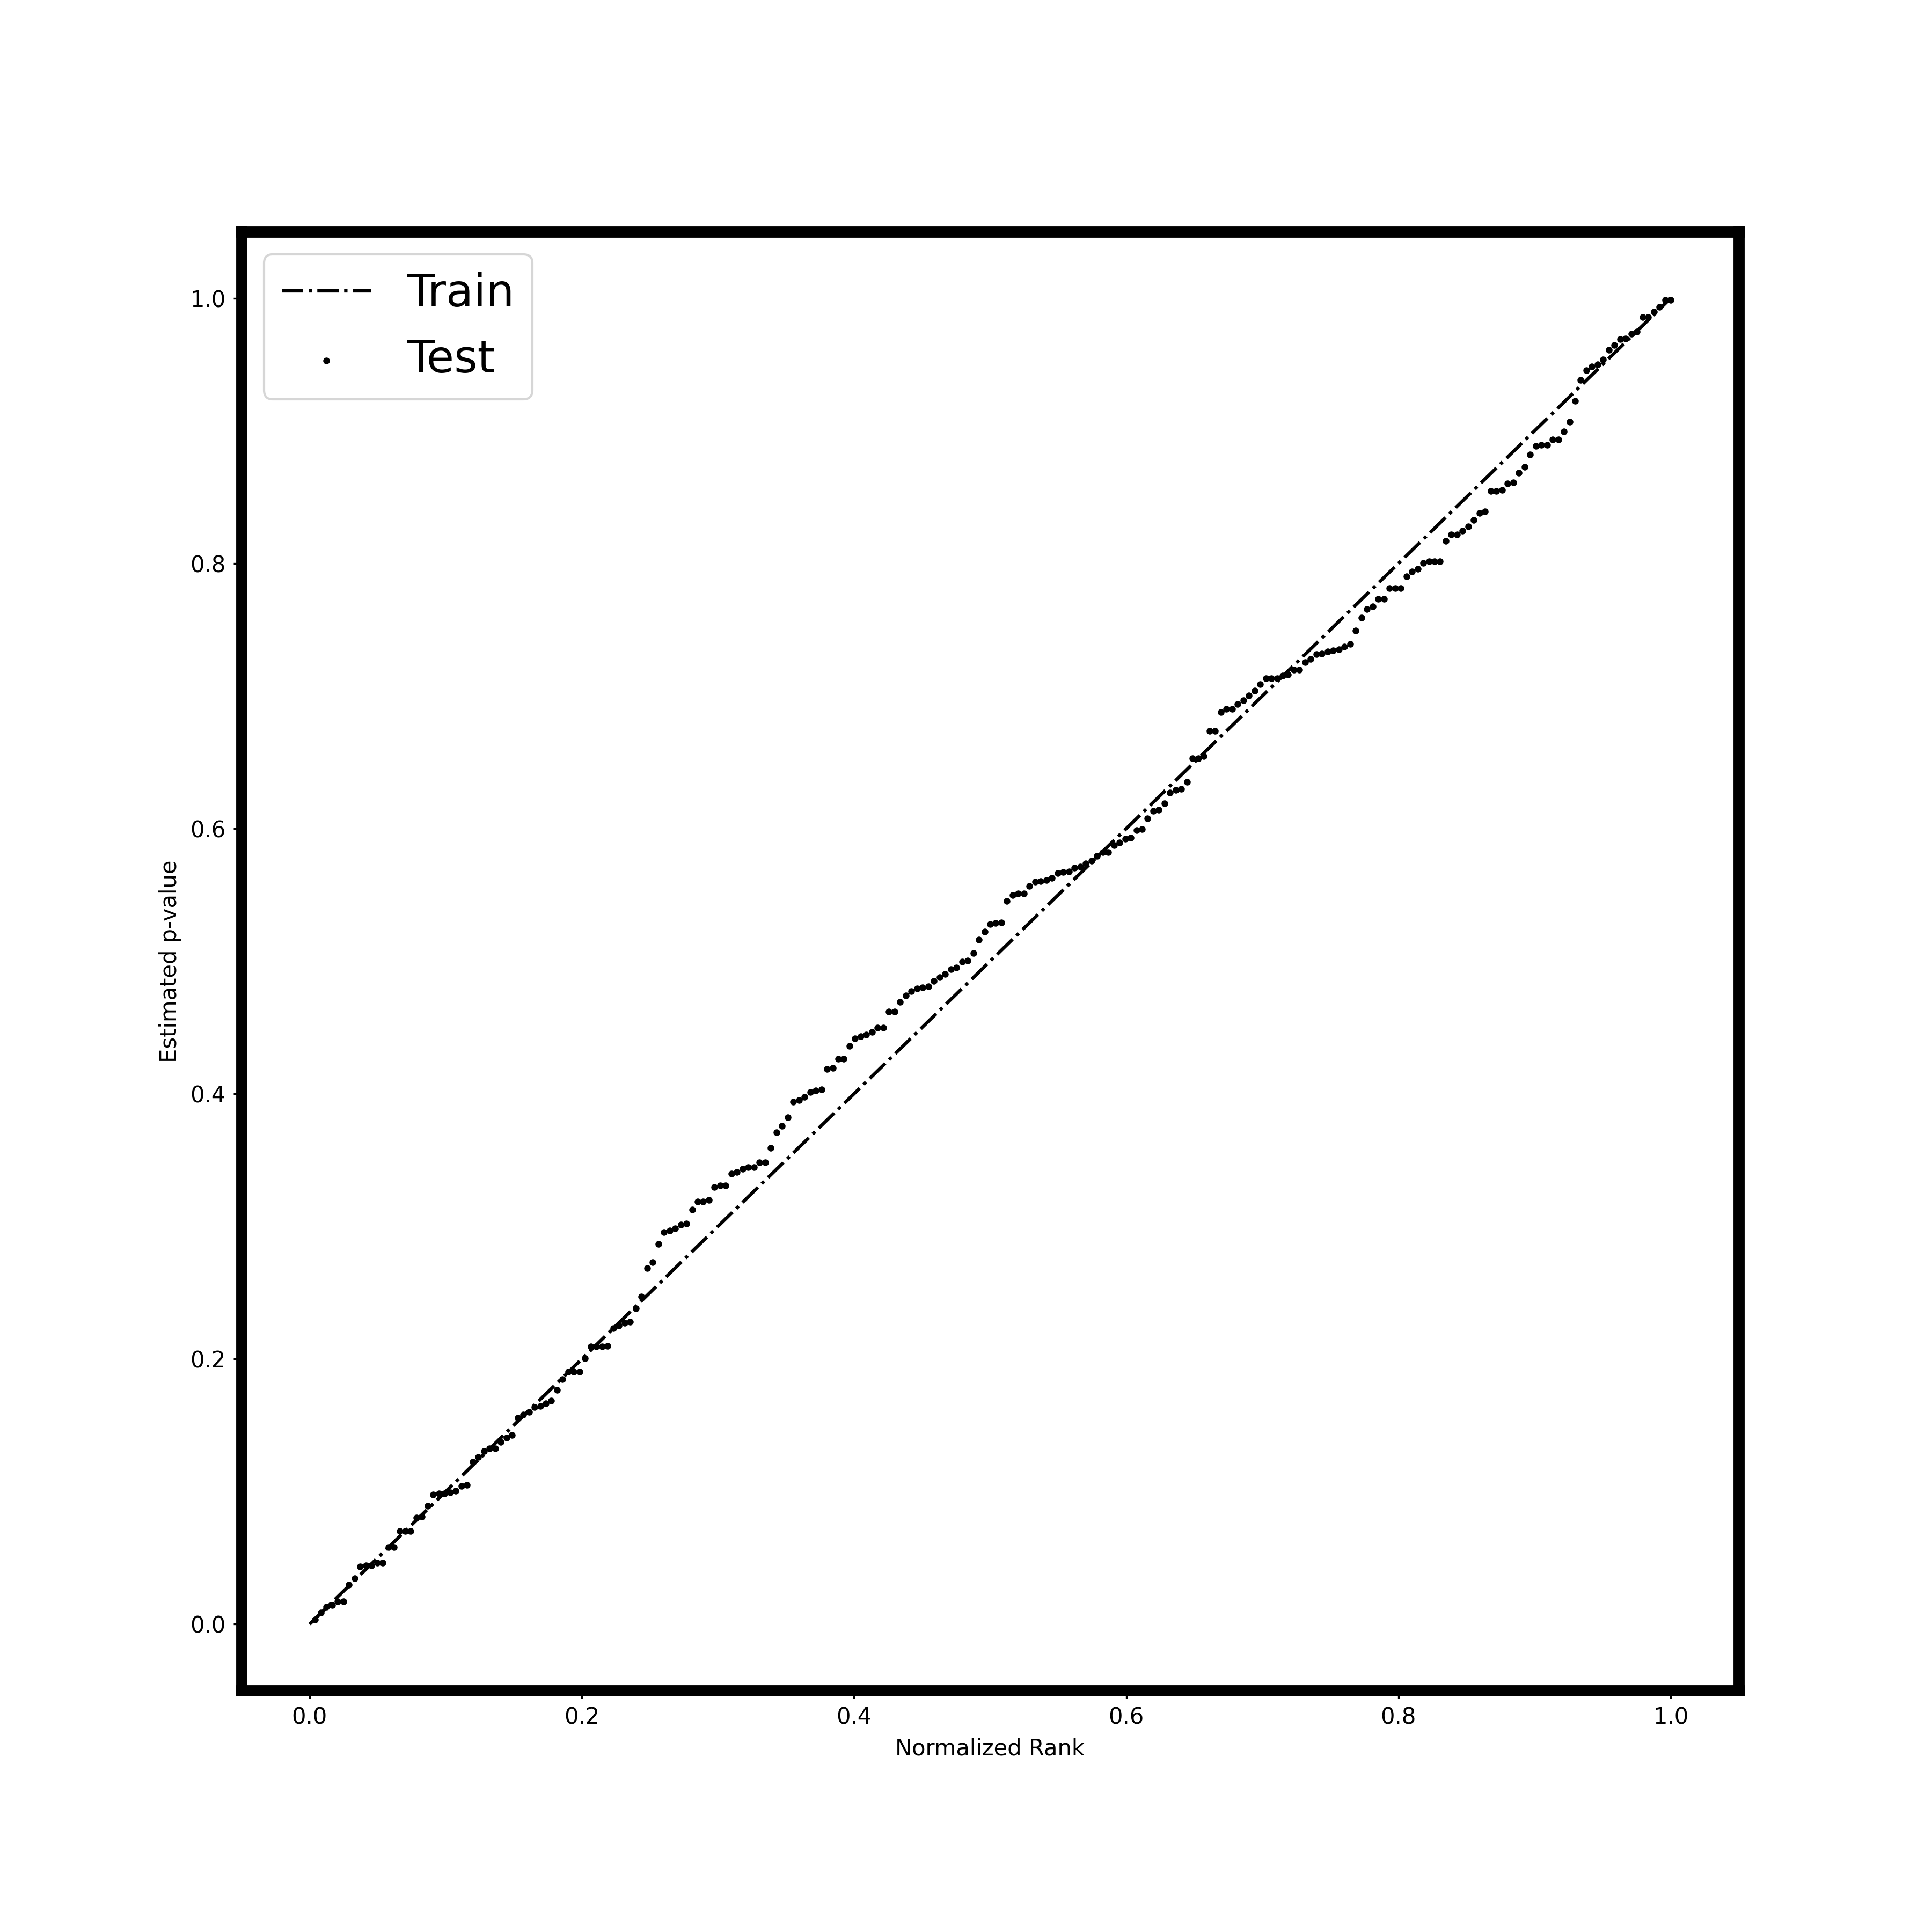
\includegraphics[width=2in]{img/cnn_QQ_multi.png} &
		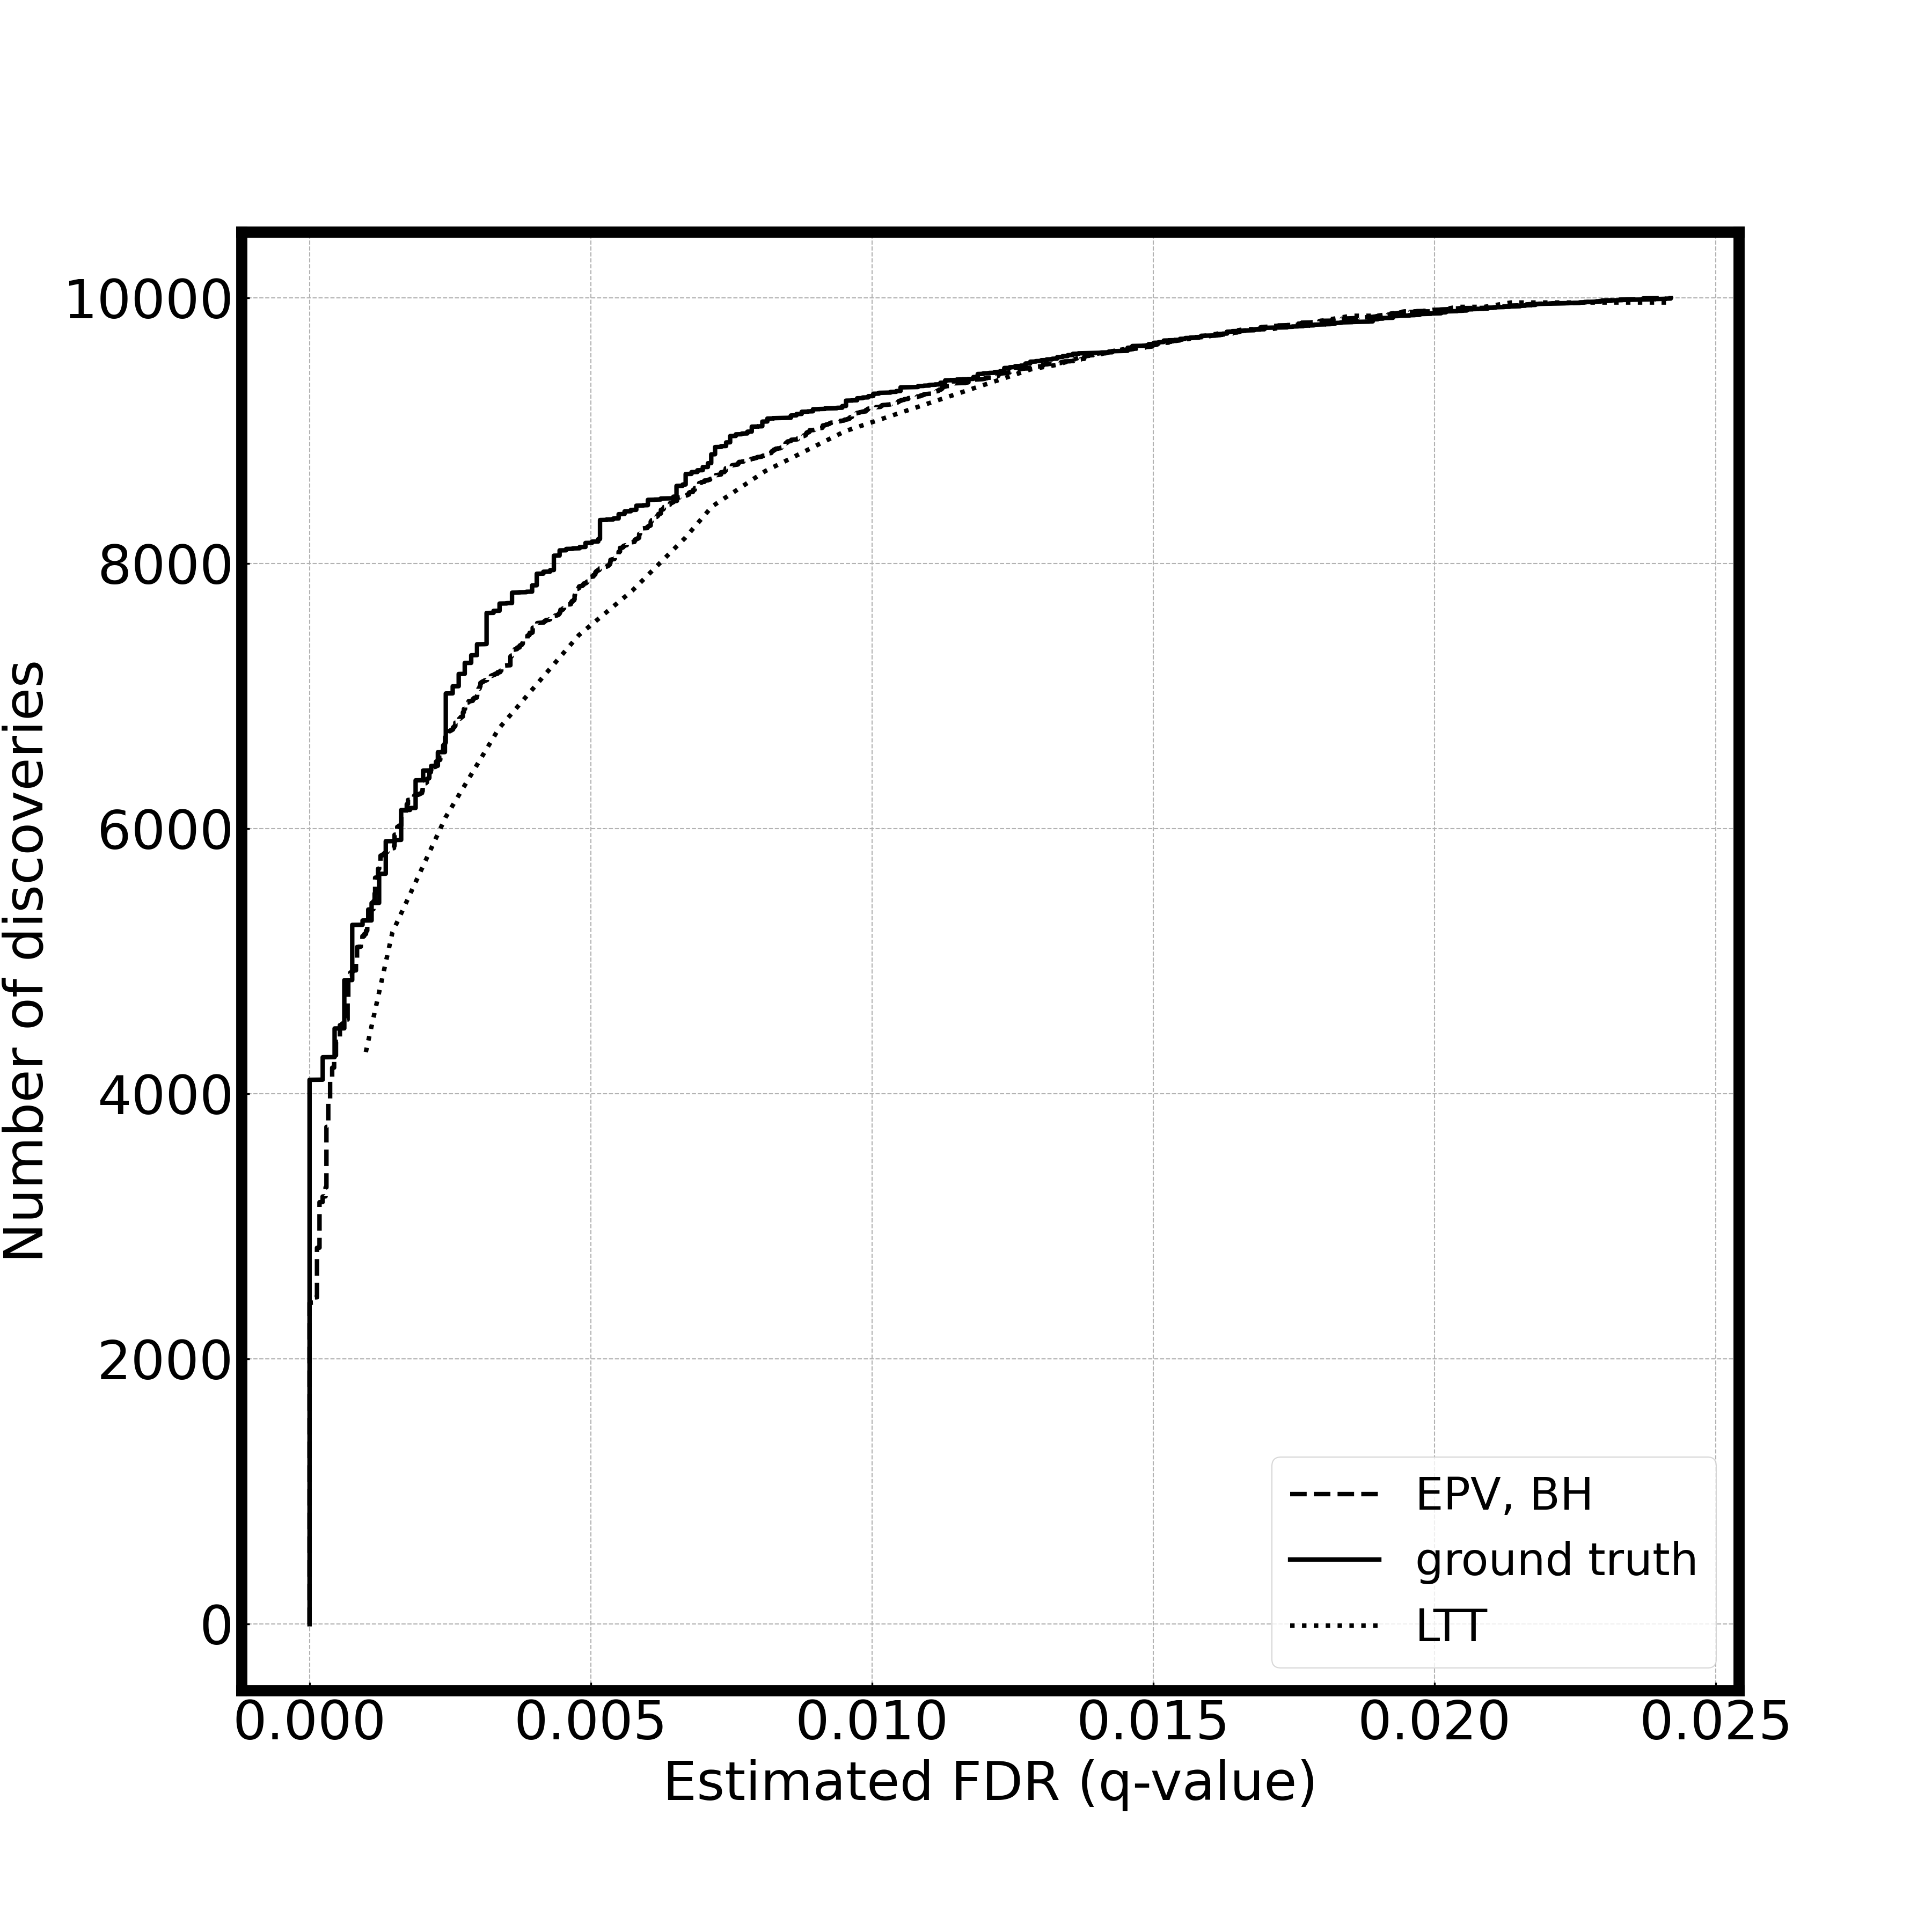
\includegraphics[width=2in]{img/cnn_test_pred_multi.png} \\	
		A & B \\
	\end{tabular}
	\caption{{\bf FDR control with p-values for multi-class classification.}
		(A) a QQ plot of the p-values obtained with using negative training data. (B) The number of trusted classifications as a function of the FDR when it is controlled with true labels (red line) and with controlled with BHP (black line) using the p-values from panel (A).
		(A) a QQ plot of the p-values obtained with using training data classified as negative. (B) The same as panel (B), but using p-values from panel (C).
	}
	\label{fig:examples}
\end{figure}


\begin{figure}
    \centering
        \begin{tabular}{ccc}
 		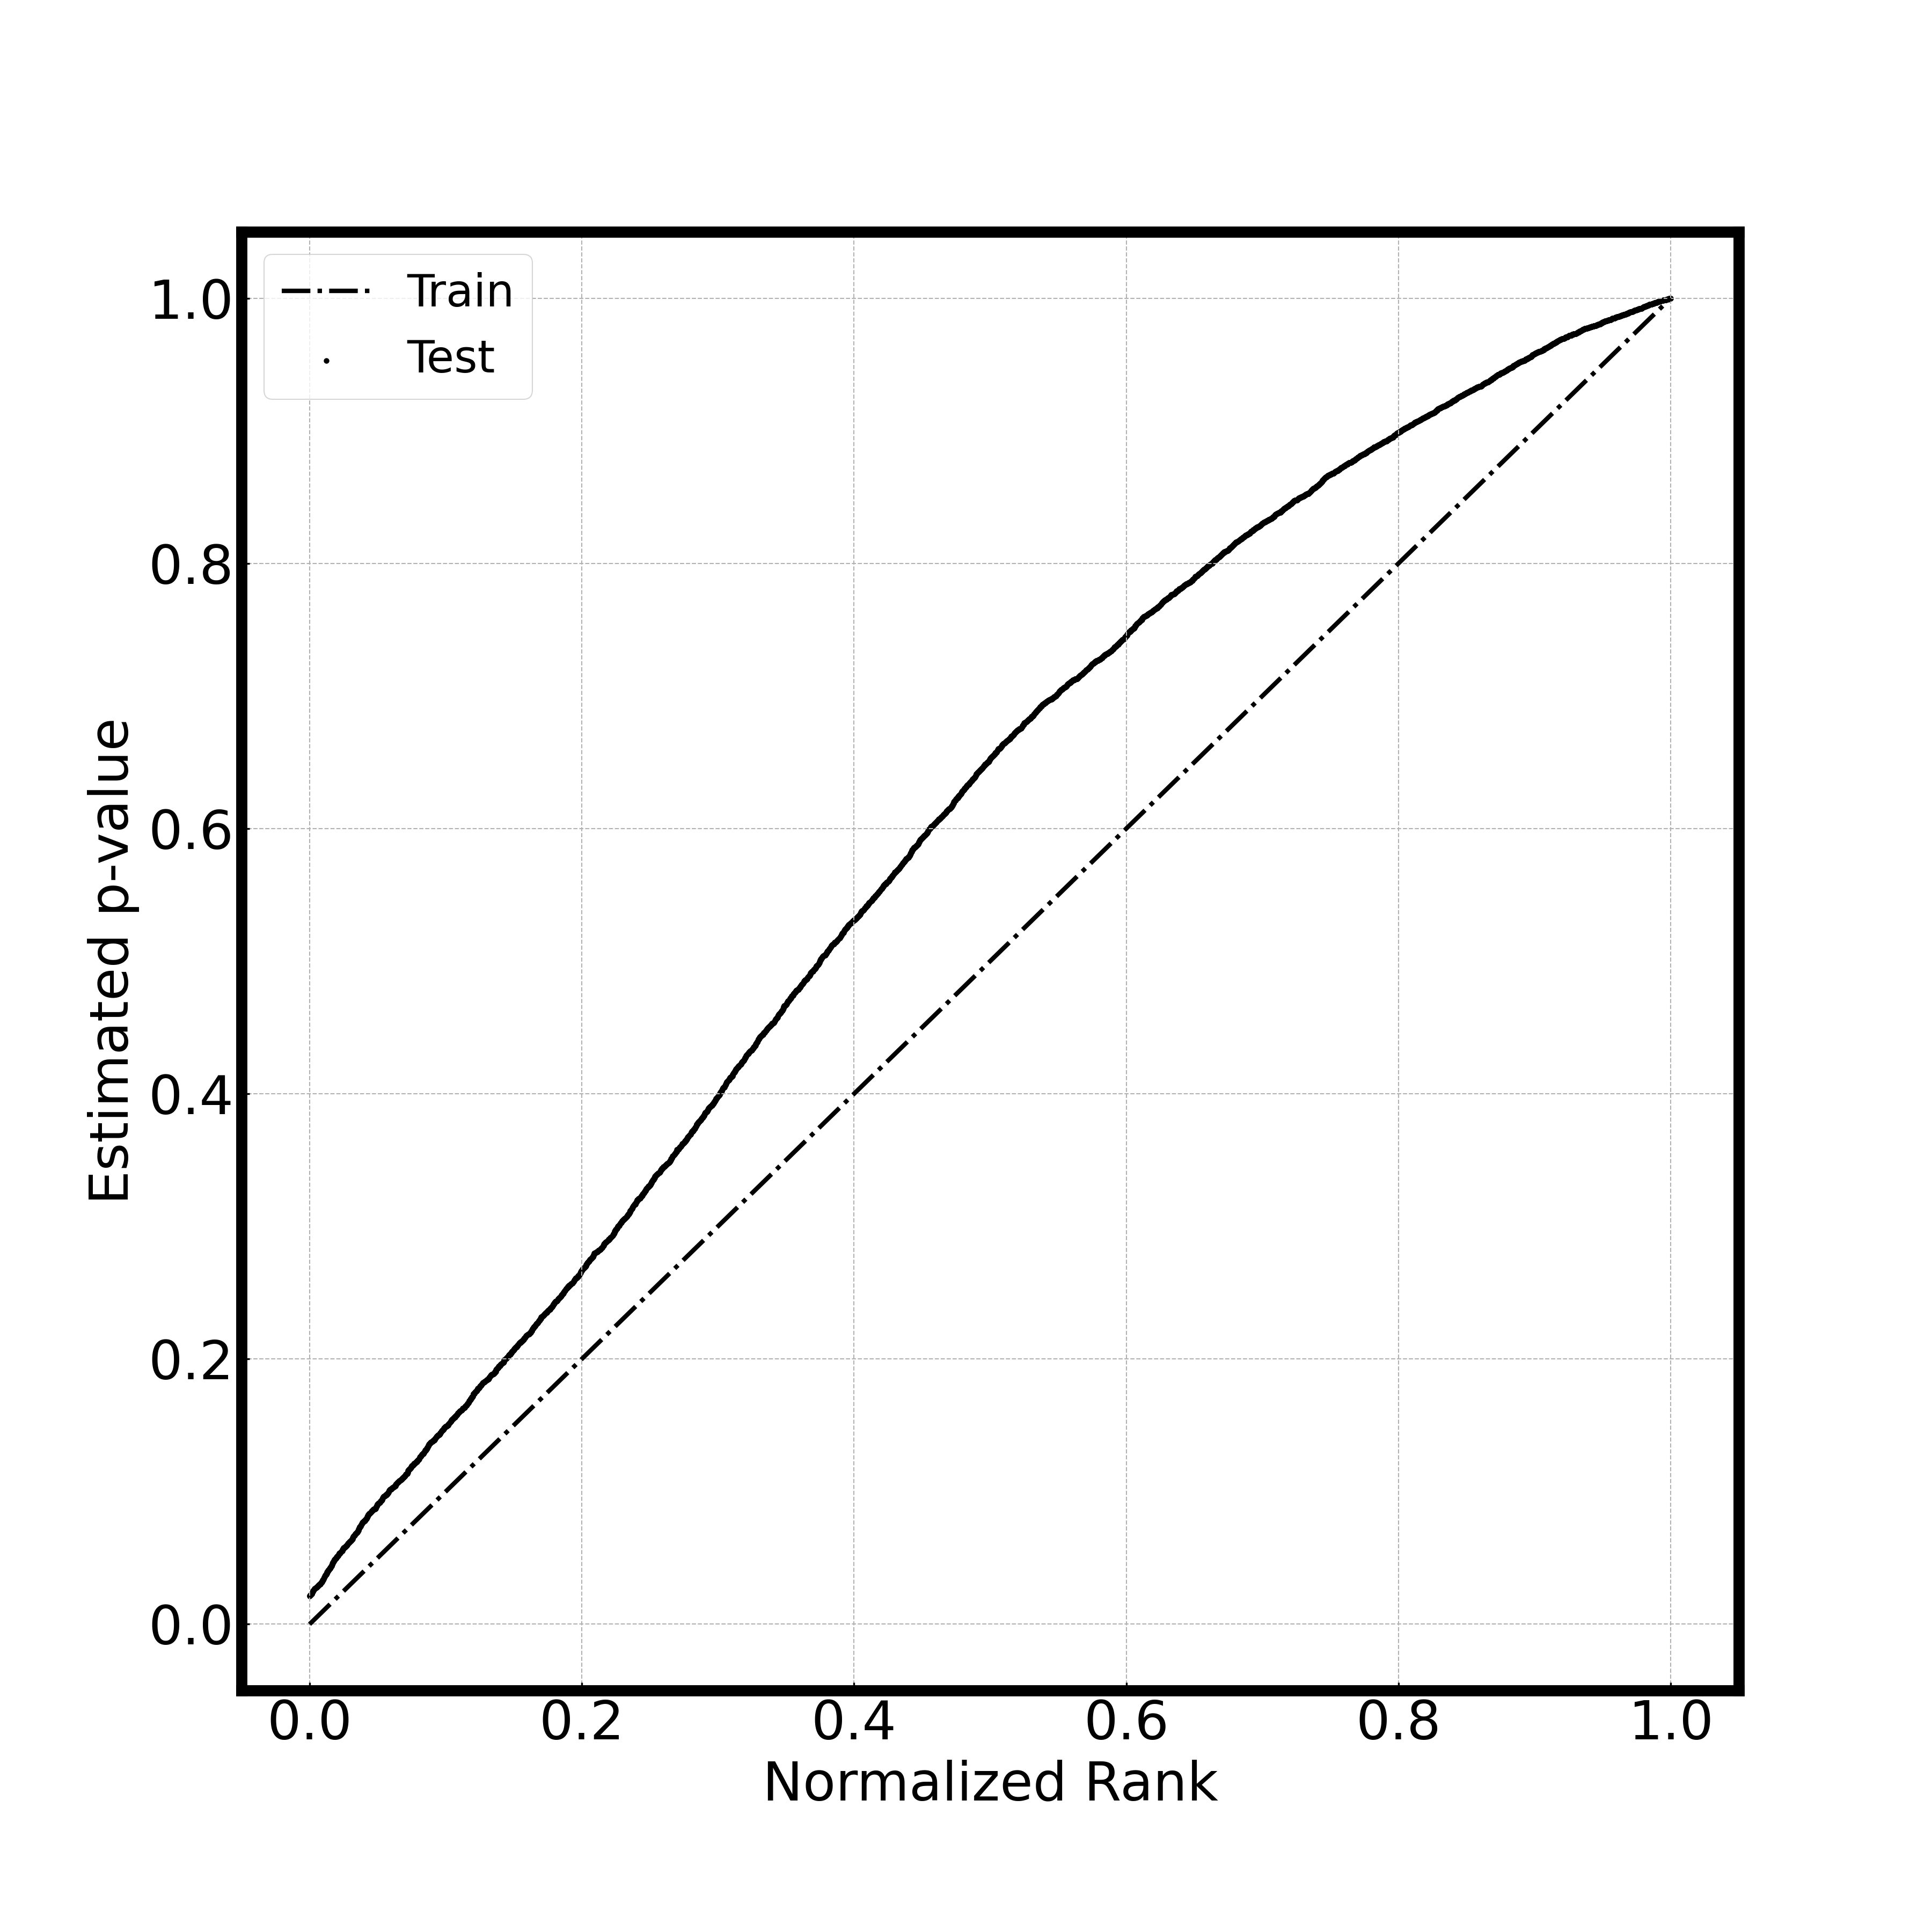
\includegraphics[width=2in]{img/cnn_QQ_shift_binary_with.png} &
		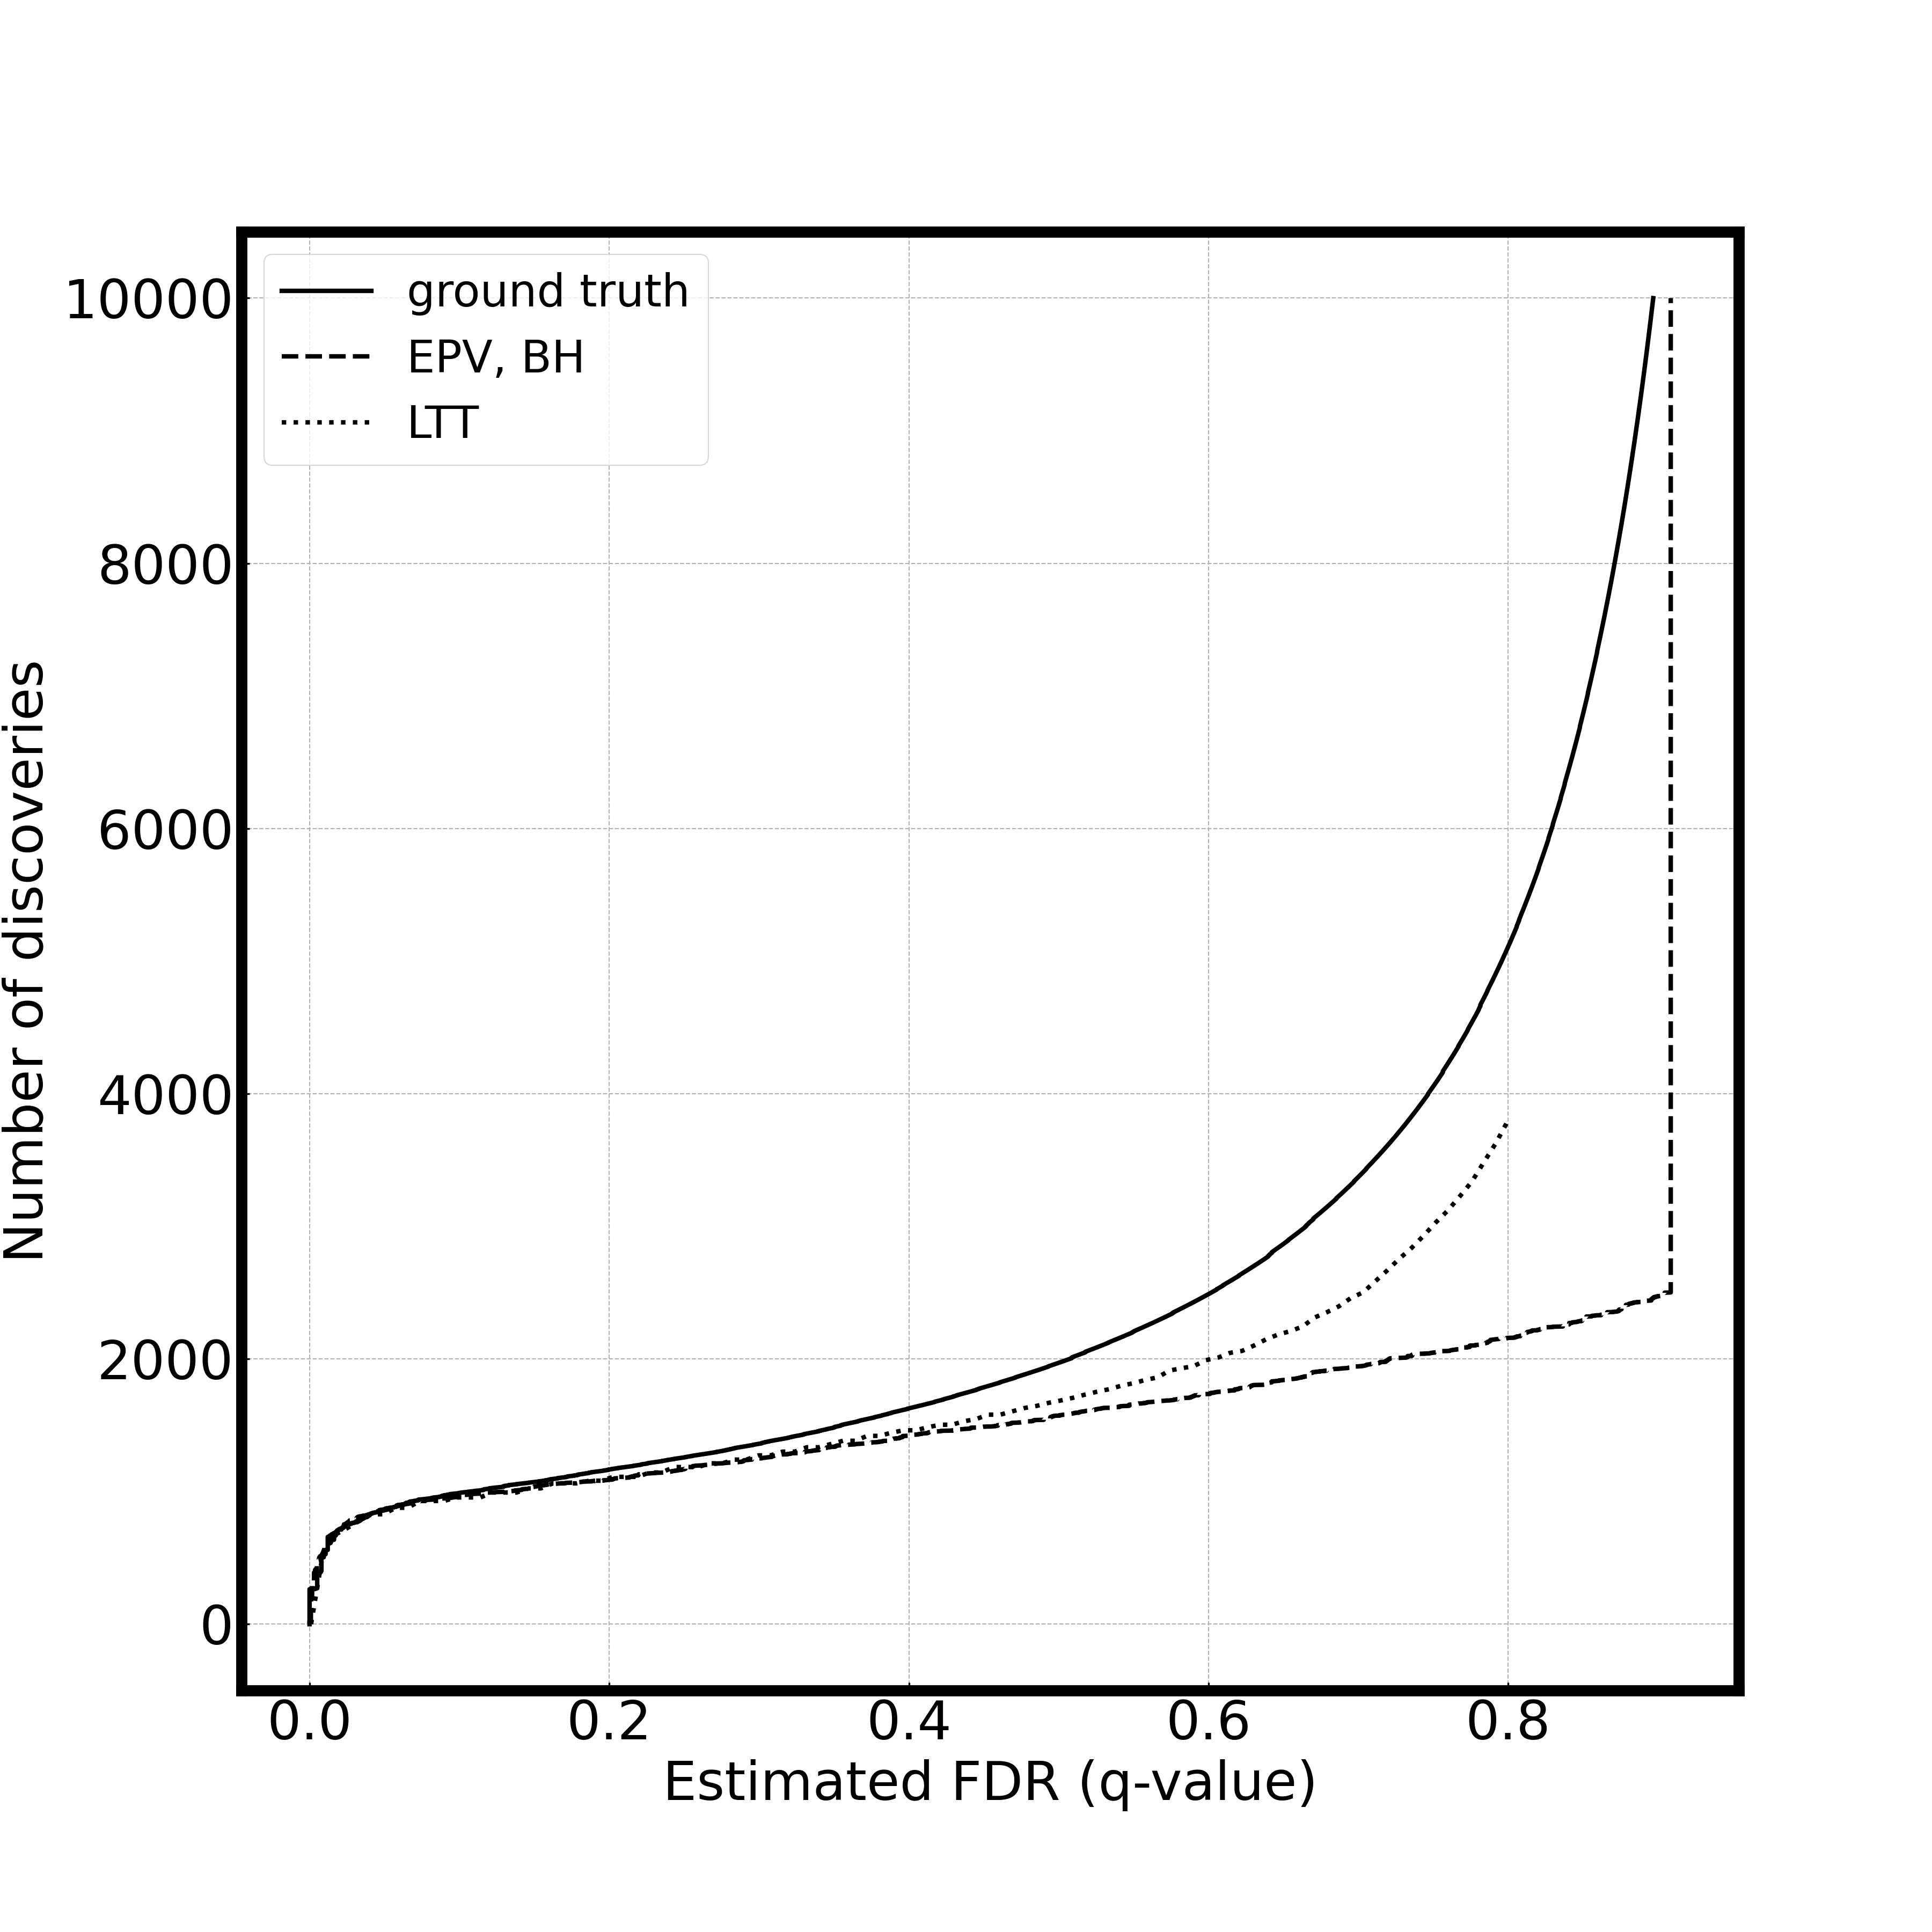
\includegraphics[width=2in]{img/cnn_shift_test_pred_with_labels.png} & 
            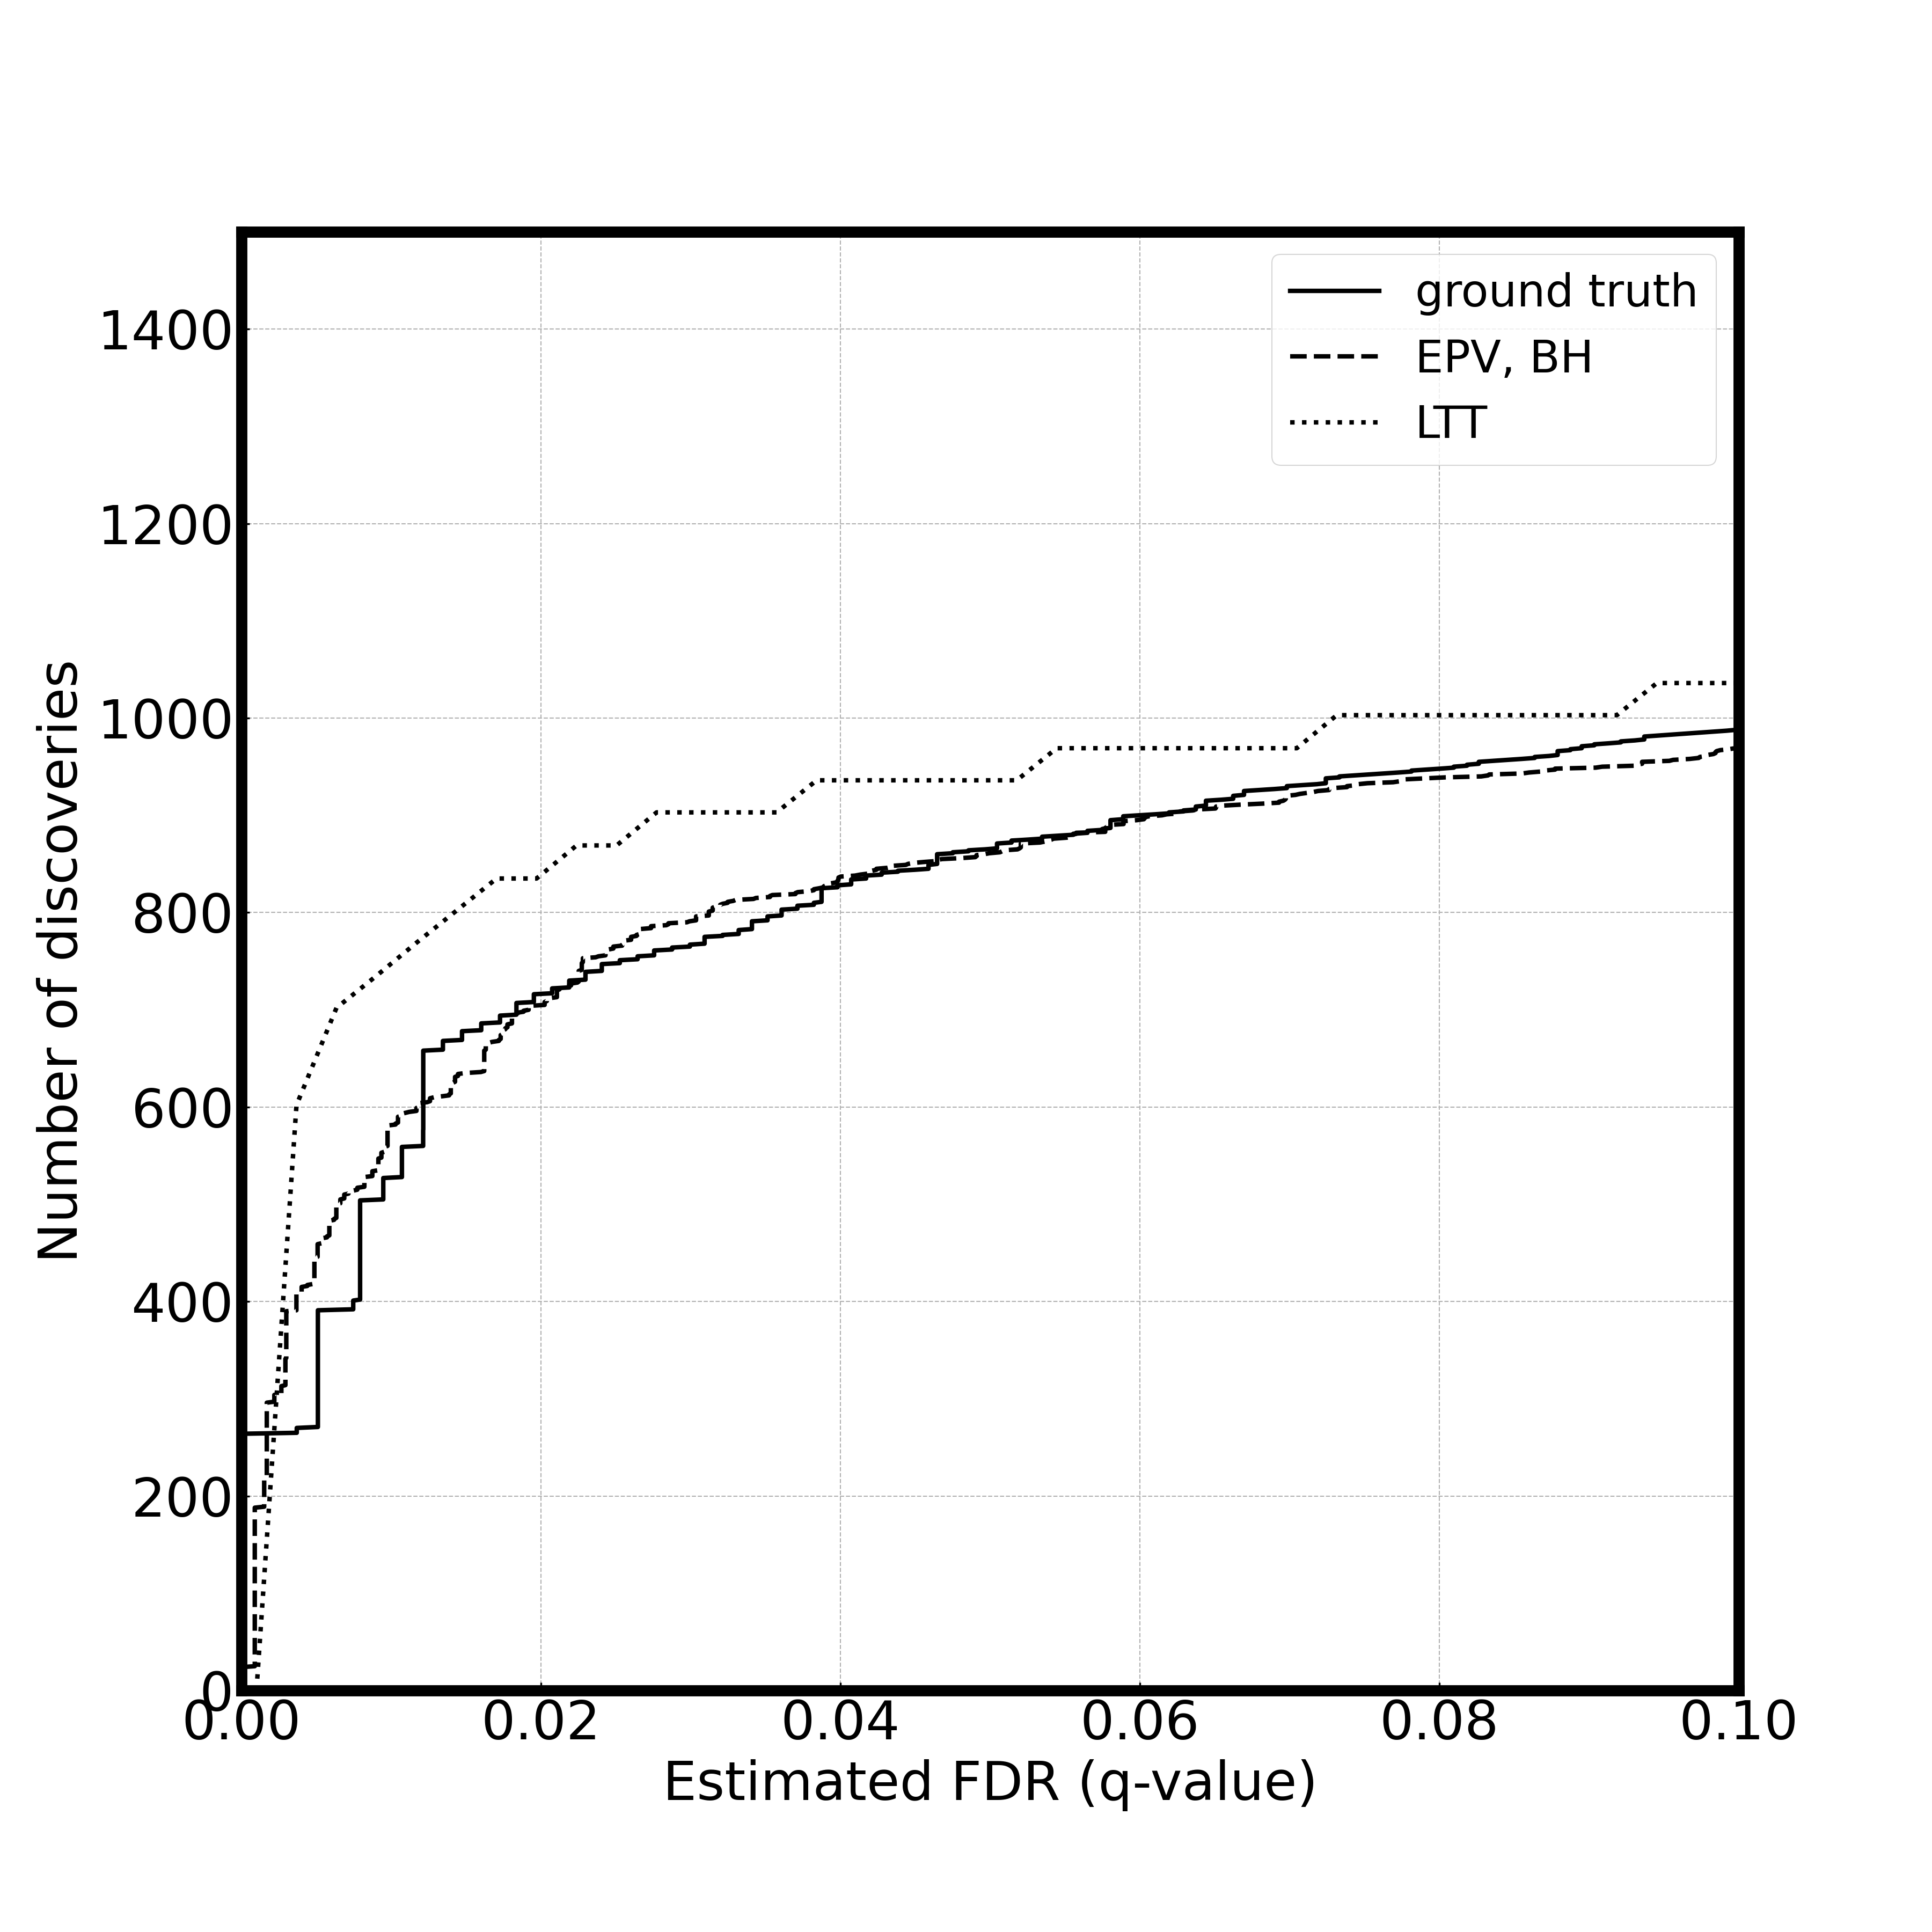
\includegraphics[width=2in]
            {img/cnn_shift_test_pred_with_labels_loc.png}
		\\	
		A & B & C\\
            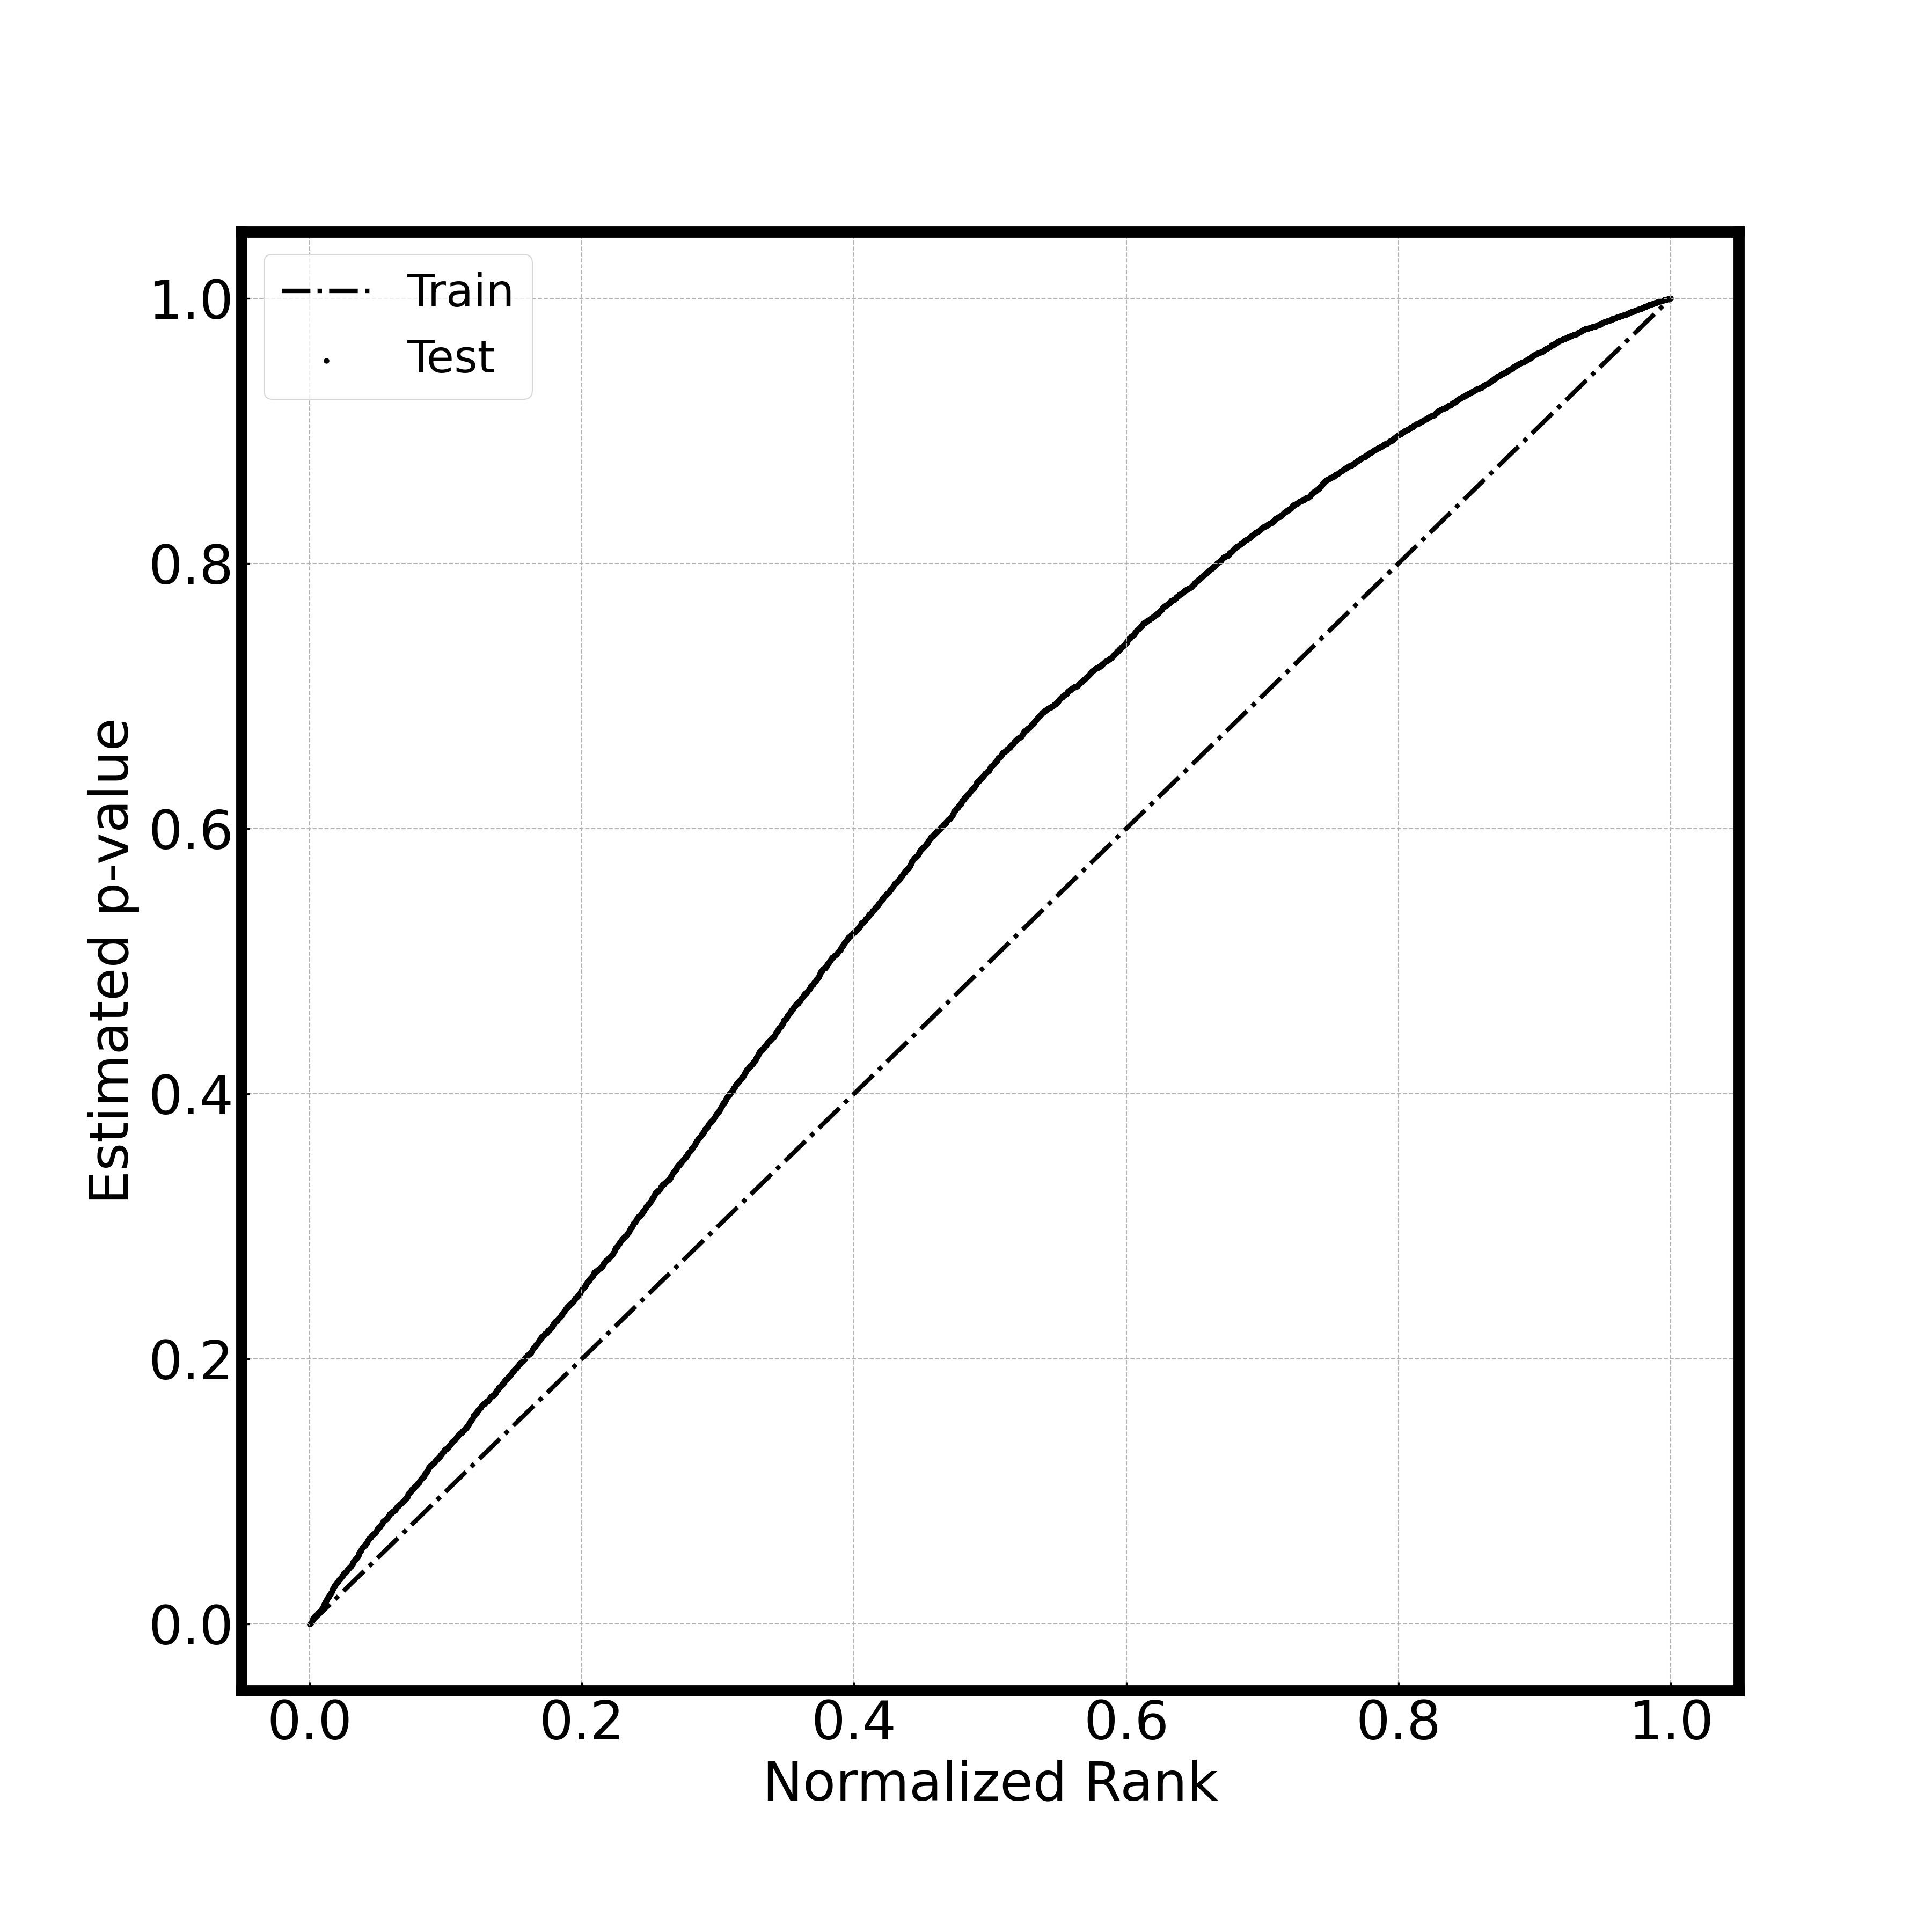
\includegraphics[width=2in]{img/cnn_QQ_shift_binary_no.png} &
		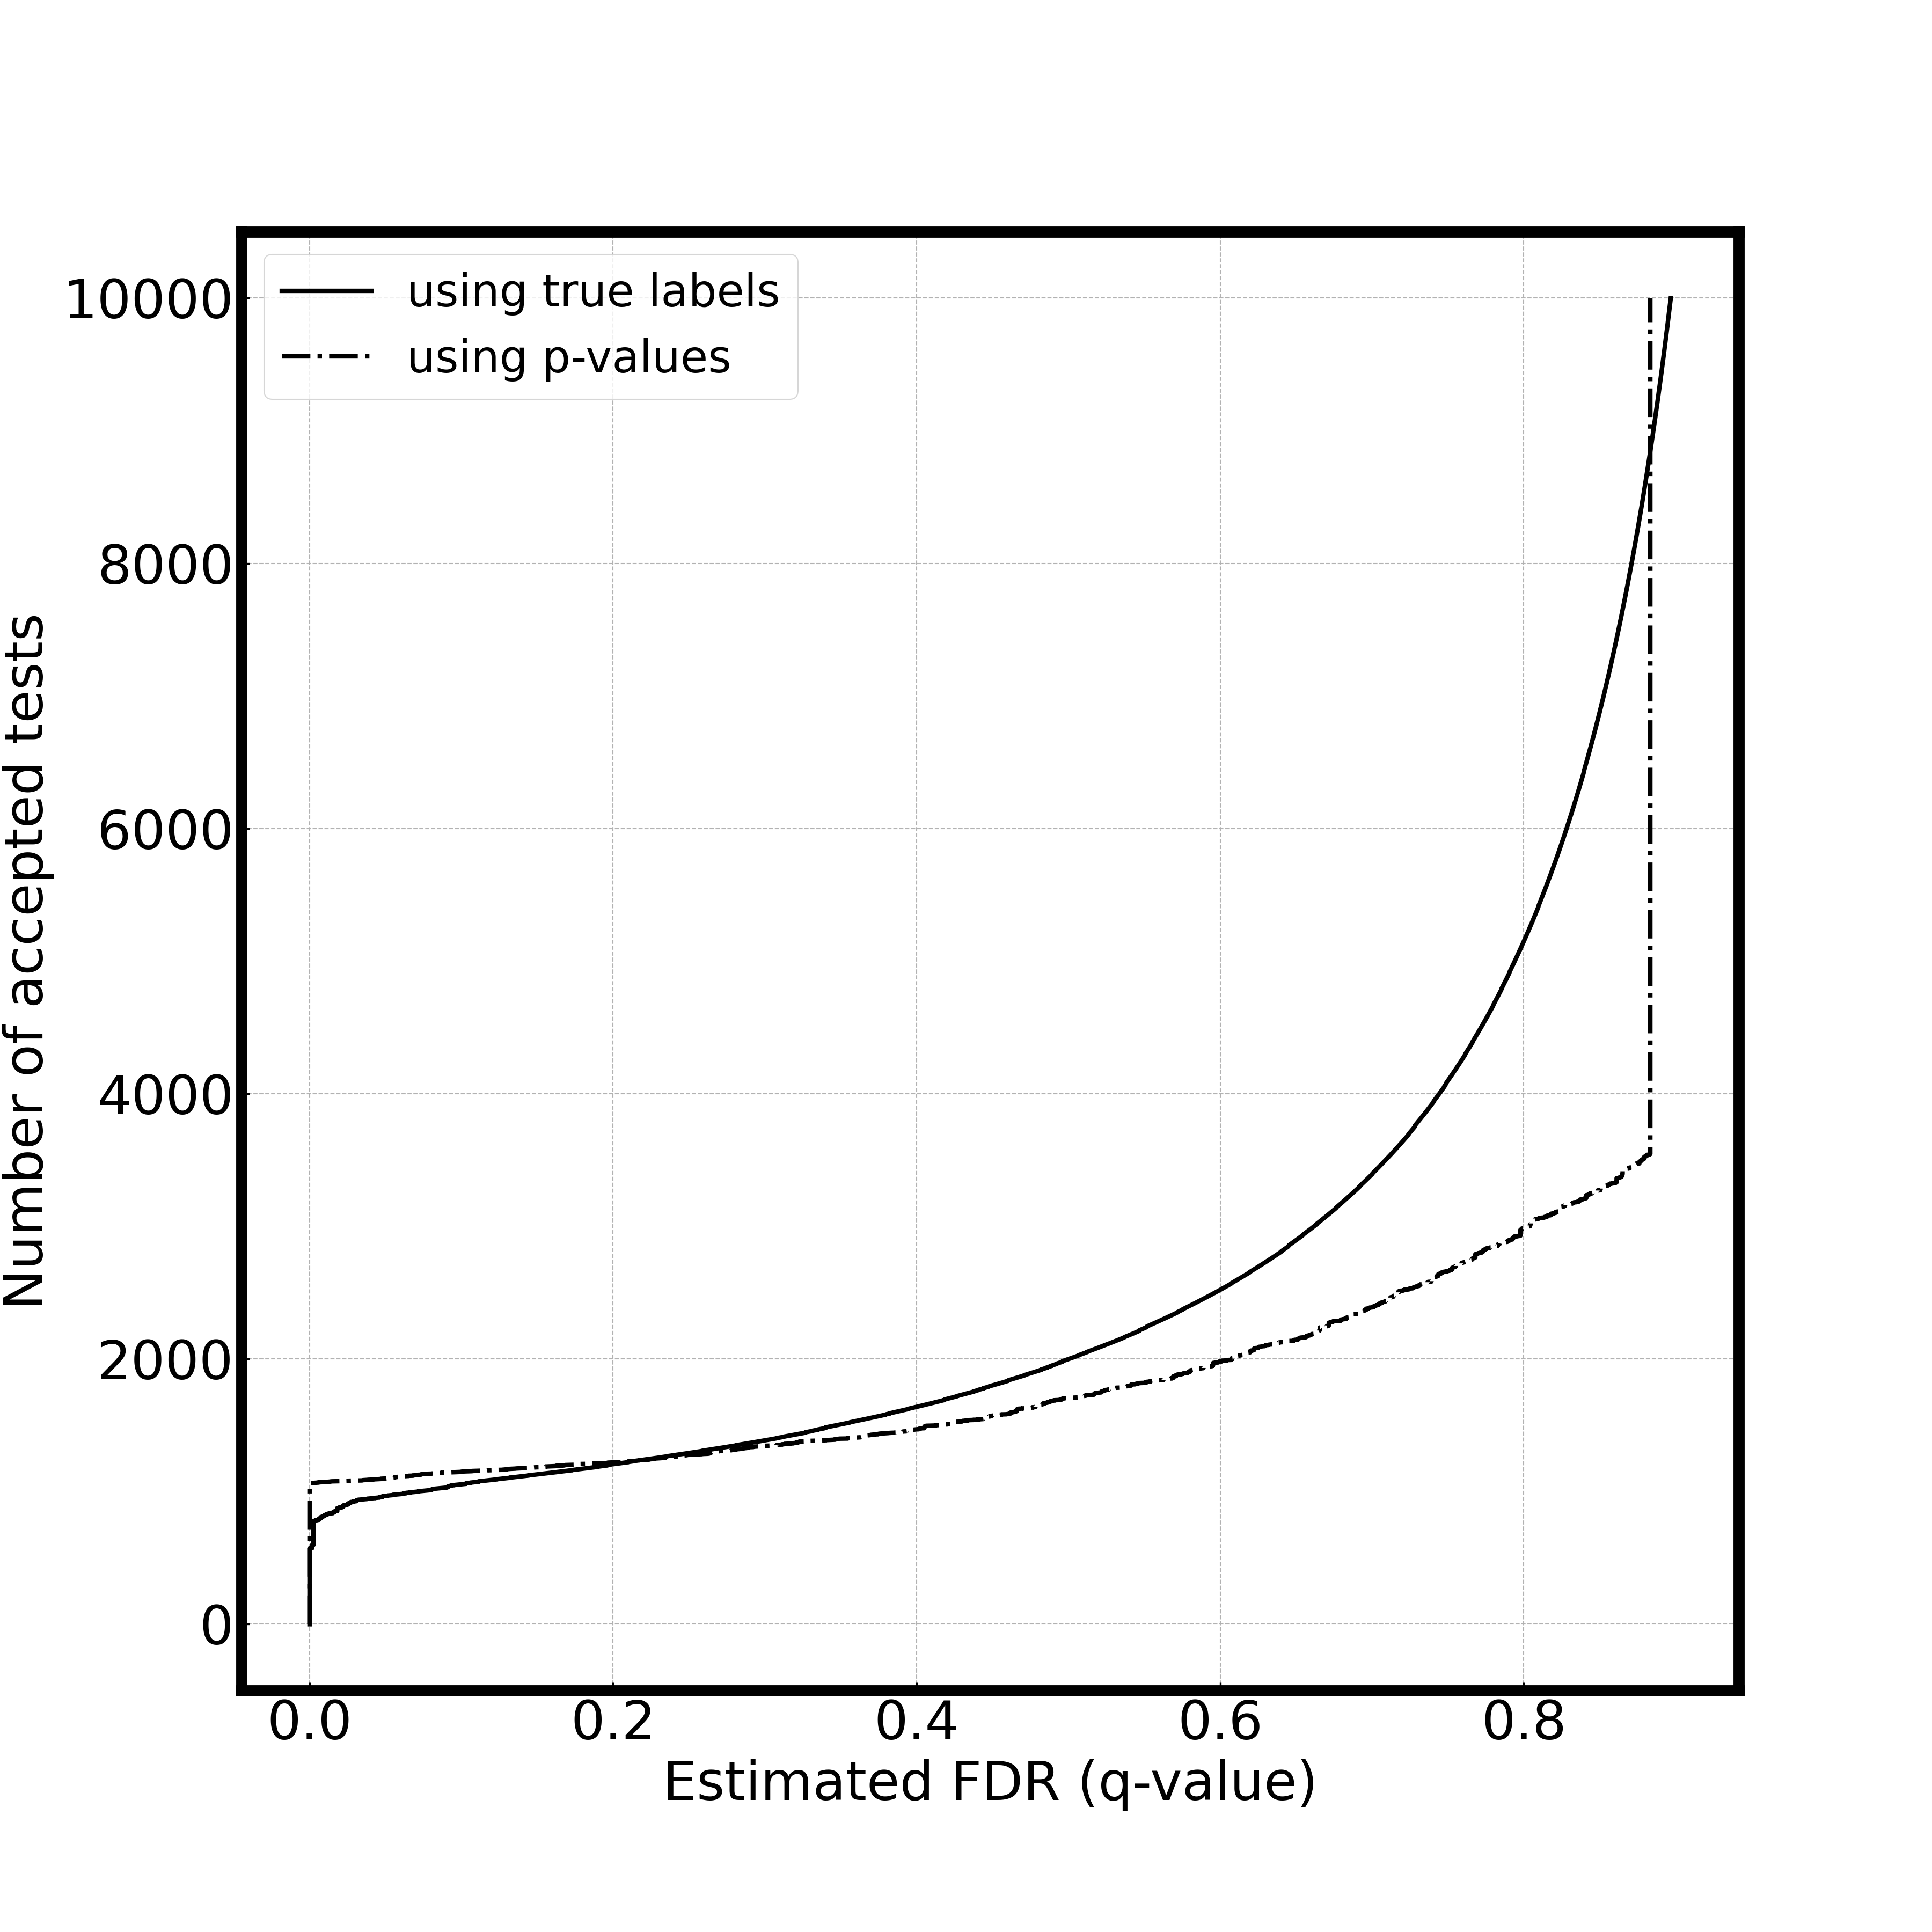
\includegraphics[width=2in]{img/cnn_shift_test_pred_no_labels.png} &  
            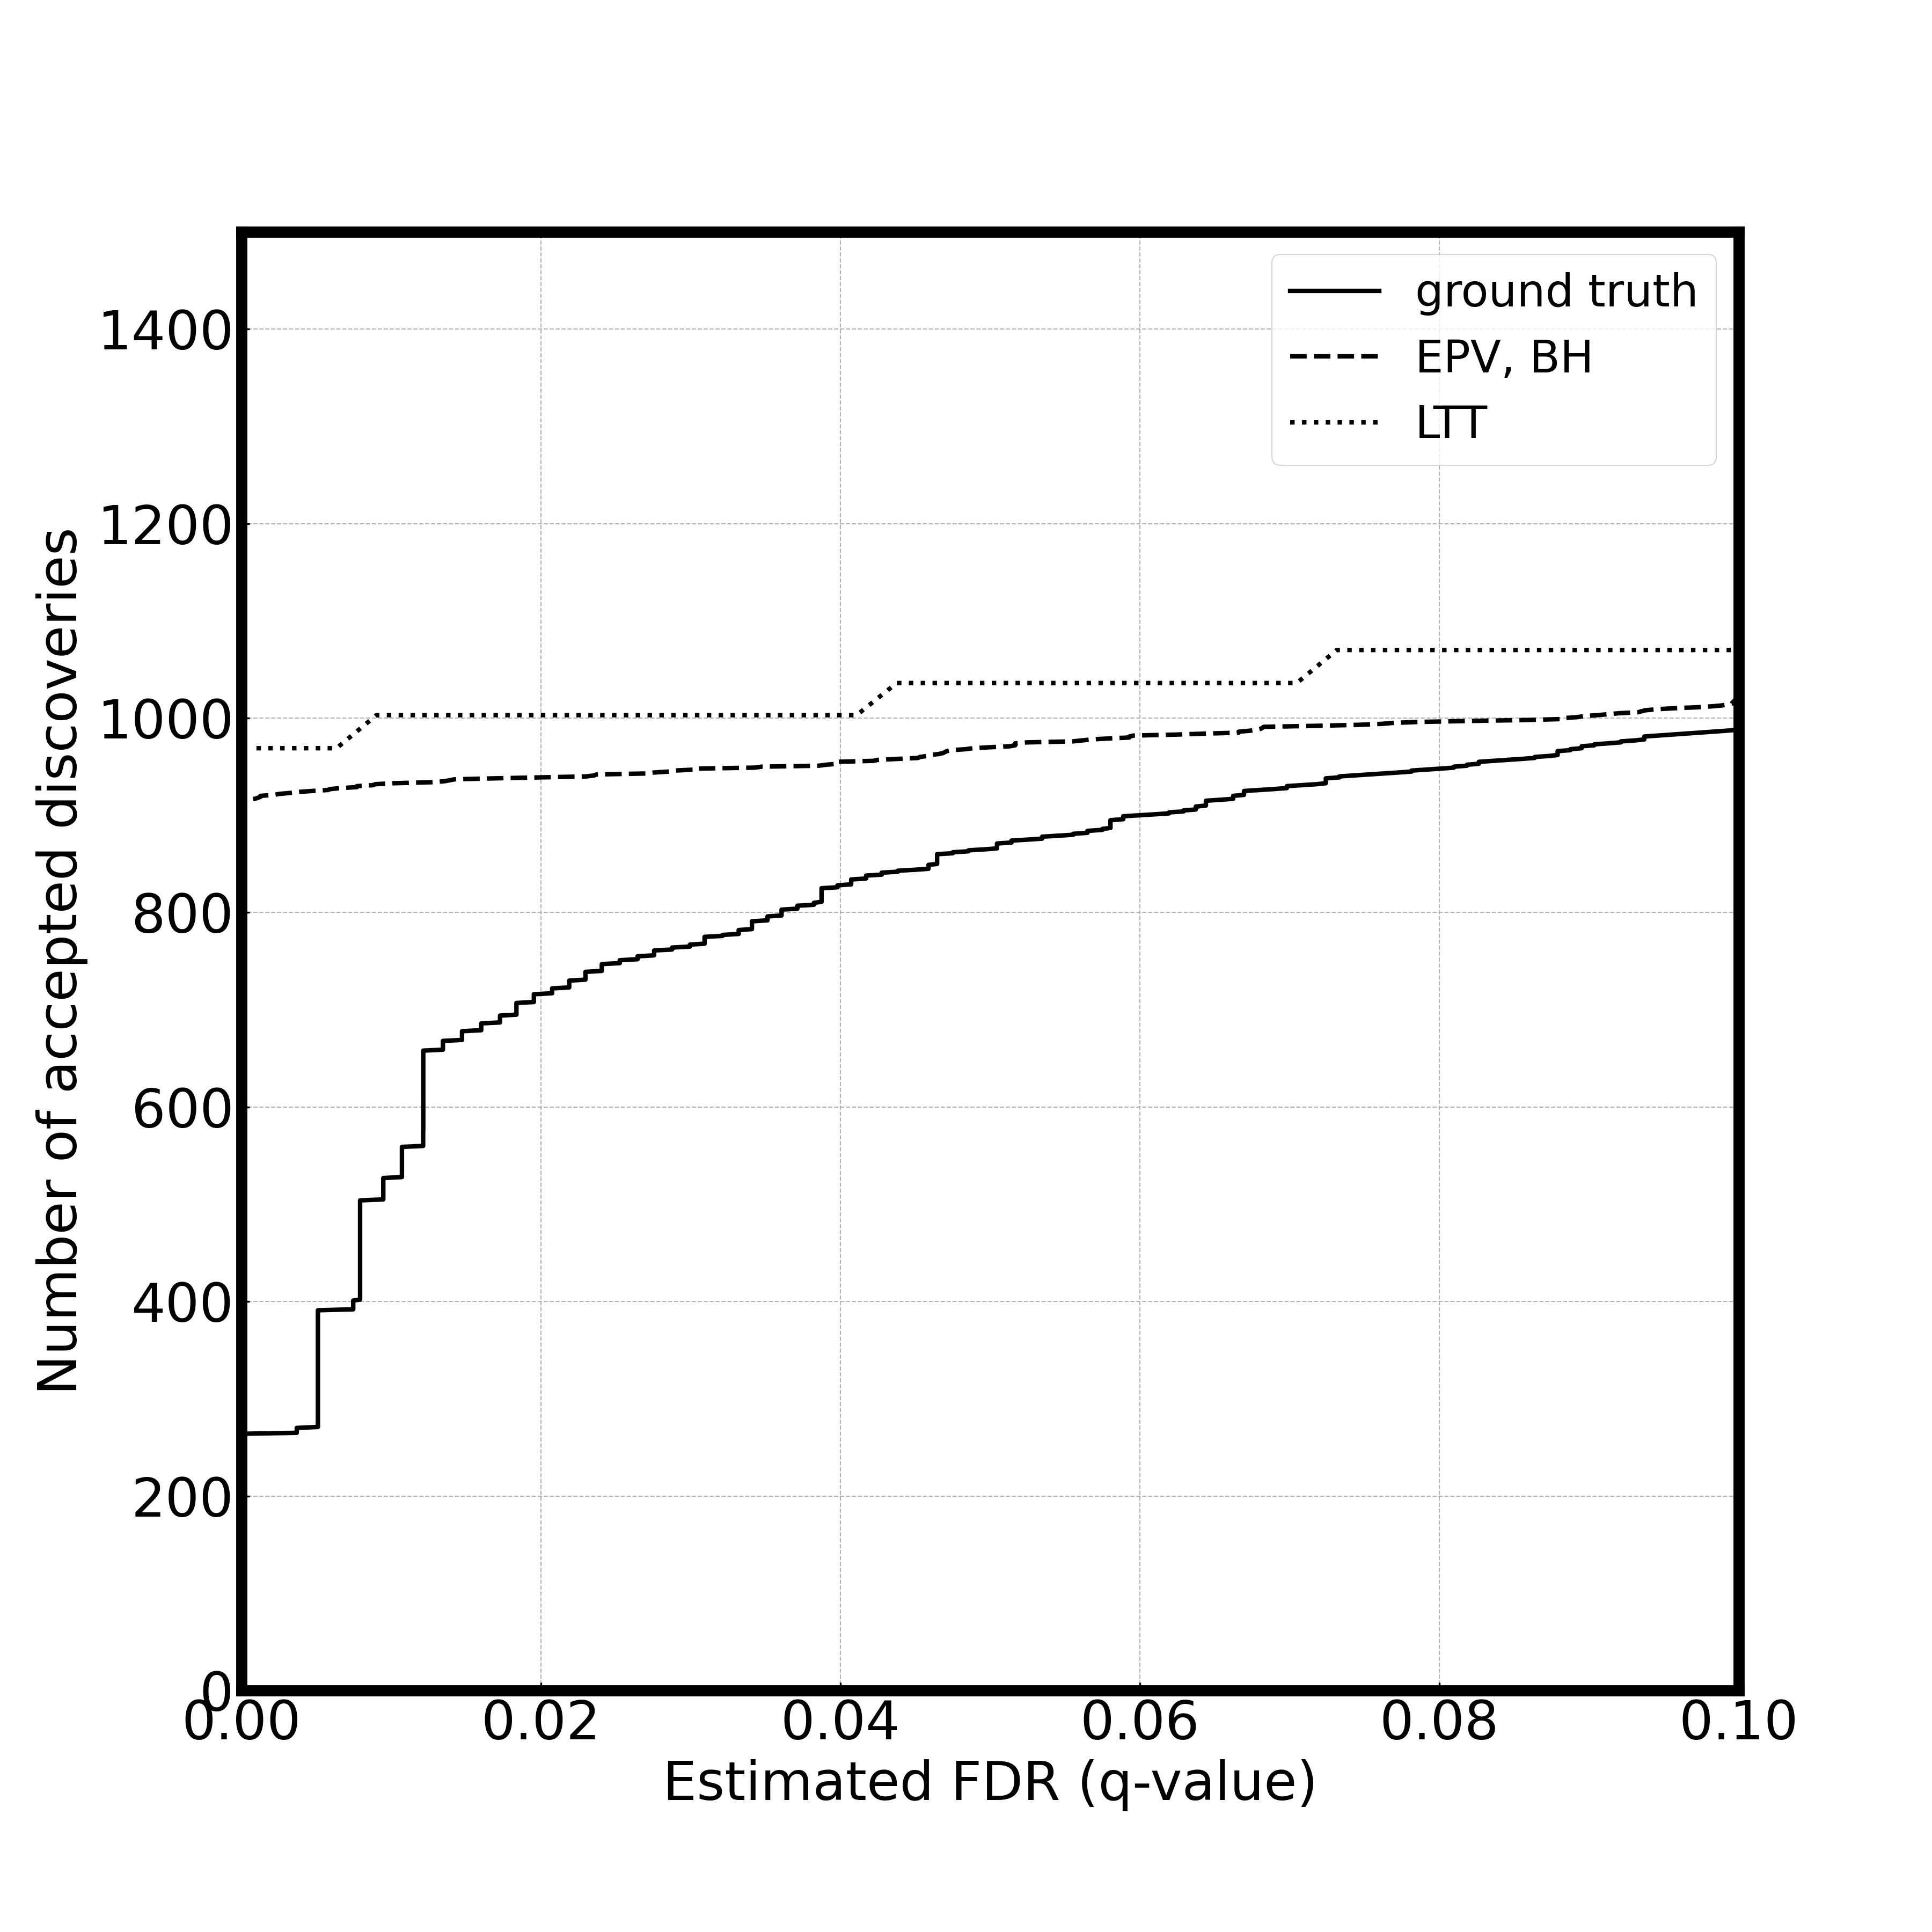
\includegraphics[width=2in]{img/cnn_shift_test_pred_no_labels_loc.png}  \\
		D & E & F \\
	\end{tabular}
	\caption{{\bf  FDR control with p-values for detecting data distribution shift.}
		(A) a QQ plot of the p-values obtained with using negative training data. (B) The number of trusted classifications as a function of the FDR when it is controlled with true labels (red line) and with controlled with BHP (black line) using the p-values from panel (A).
		(A) a QQ plot of the p-values obtained with using training data classified as negative. (B) The same as panel (B), but using p-values from panel (C).
	}
	\label{fig:examplesssss}
\end{figure}


\subsection{p-values for multi-class classification}

For multi class classification, the p-value indicates significance of that a sample is correctly classified. The null distribution is constructed from the miss-classified training data. Therefore, we aim to control that whether a test data is correctly classified to its class or not. The $\pi_0$, again is estimated by the proportion of the negative classification among all classifications.

\subsection{detecting data distribution shift}

For further examination of p-values’ nature, we introduced a brief experiment on data distribution shift. After training model on the MIST dataset, a 1-by-1 pixel move was performed for each image. Then the newly born samples were run through the already trained model. However, the emerged QQ plots have shown a radical alteration compared to the preceding graphs. The comparison outlines the p-values’ initial uniform distribution’s elimination. 


%
%Exact methods ... 
%Let us discuss this method in detail. This method requires the following elements:
%\begin{enumerate}
%	\itemsep-3pt  		
%	\item Mass ...
%	
%	\item Exact methods employ ...
%\end{enumerate}
%
%The XPV method begins by placing a 1.0 to the $D[n,0]$, where $n$ indicates the discretized mass of the N-terminal group. This means that, there is exactly one N-terminal residue but its corresponding score is exactly 0, because N-terminal residues are not considered in the scoring. The elements of the dynamic programming table are filled recursively. Let us consider the cell $D[r,c]=n$, where there are exactly $n$ peptide fragments whose discretized mass is $c$ and they all score exactly $r$. Consequently, when all of these $n$ different peptide fragments are appended with an amino acid $X$, then there are $n$ peptides with a discretized mass of 
%\begin{equation}
%b=c+d_w(X)
%\label{eq:new_column}
%\end{equation}
% and their score
%
%\section{Data sets and methods}
%
%
%\subsection{Data sets}
%In our experiments, we used four, publicly availabl
%
%\begin{table}[t]
%	\centering
%	\caption{Summary of mass spectrometry data sets}
%	\label{tb:dataset_ms_summary}
%	\begin{tabular*}{\textwidth}{l@{\extracolsep{\fill}}llrr} 
%		\hline
%		ID& Name&Instrument& Num. of spectra & ACP$^1$\\
%		\hline
%		HumVar & H. Sapiens, Human Variation& LTQ Orbitrap& 15,057 & 2771.89  \\
%		Malaria& P. Falciparum & LTQ Orbitrap& 12,594  & 1024.06\\	
%		Kingdom& H. Sapiens  & Q Exactive HF-X Orbitrap	&  178,024& 2124.93\\
%		LUAD &  H. Sapiens, Lung Adeno Carcinoma & Q Exactive HF-X Orbitrap & 41,613 &2771.92\\
%		\hline		
%	\end{tabular*}\\
%	\raggedright \footnotesize Notes: The precursor ion tolerance was set to 10 ppm for all data sets, no isotope error was allowed. $^1$Average candidate peptide per spectrum.
%\end{table}
%
%\section{Results and discussion}
%\subsection{Main results}
%We begin 
%\begin{figure}[h]
%   \centering
%   \footnotesize
%   \setlength{\tabcolsep}{0pt}	
%  % \begin{tabular}{cc}	
%%		(A)\raisebox{-0.90\height}{\includegraphics[trim=0cm 0cm 0cm 0cm,clip=true, width=0.45\textwidth]{HUMVAR.pdf}} &
%%		(B)\raisebox{-0.90\height}{\includegraphics[trim=0cm 0cm 0cm 0cm,clip=true, width=0.45\textwidth]{MALARIA.pdf}}\\ 
%%		(C)\raisebox{-0.90\height}{\includegraphics[trim=0cm 0cm 0cm 0cm,clip=true, width=0.45\textwidth]{KINGDOM.pdf}}& 
%%		(D)\raisebox{-0.90\height}{\includegraphics[trim=0cm 0cm 0cm 0cm,clip=true, width=0.45\textwidth]{LUAD.pdf}} \\
%%	\end{tabular}
%\caption{The number of PSMs accepted at various FDR levels obtained with refactored XCorr, Tailor, and XPV methods using HRFS and LRFS in our benchmark data sets.}
%\label{fg:hrxpv-perf}
%\end{figure}

\section{Conclusions}
The original exact p-value (XPV) calculation methods for scoring tandem mass spectrometry data using a dot-product-like scoring function were introduced for low-resolution fragmentation settings almost 15 years ago. Until now, it has remained an open question whether this algorithm can be made suitable for high resolution fragmentation settings. In this article we showed a generalization of the XPV method, termed HR-XPV, which is capable of producing accurate and well calibrated exact p-values for XCorr scores obtained with scoring high resolution MS/MS data. Unfortunately, our solution can be considered rather slow, which raise questions about its practicality. However, we hope that, the ideas in HR-XPV presented might be a significant step toward the development of efficient methods for calibrating exact p-values for high resolution MS/MS data. 

\section*{Author contributions}
\ifdefined\DOUBLEBLINDREVIEW
Omitted for double-blind peer-review.
\else
AKF concieved the idea that accurate empirical p-values would be derived from training data. AB worked out the methods and carried out experiments. AKF and AB wrote the manuscript.
\fi

\section*{Competing financial interests}
The authors declare no competing financial interests.


\section*{Availability}
\todo{AB}{Prepare a github page with the jupyter notebook experiments.}

%
%\begin{suppinfo}
%	The following supporting information is available free of charge at ACS website \url{http://pubs.acs.org}.
%	\begin{itemize}		
%		\itemsep0cm 	
%		\item Supplementary Note S1: Detailed description of the experimental data used. 
%		\item Supplementary Note S2: Detailed description of the methods used.
%		\item Supplementary Algorithm S1: Detailed pseudo code of the standard exact p-value (XPV) algorithm for XCorr scoring.
%		\item Supplementary Algorithm S2: Detailed pseudo code of the high -resolution exact p-value (HR-XPV) algorithm for XCorr scoring of high resolution MS/MS data.
%		\item Supplementary Data File S1 ({\bf \url{scripts.zip} (Zipped Linux bash scripts)}.): Script files to reproduce our experiments containing all the parameters used.
%	\end{itemize}	
%\end{suppinfo}

%\printbibliography	
\bibliographystyle{plain}           % Style BST file.
\bibliography{bibliography}

\end{document}
